%% =====================================================================
%%  M.Tech Thesis -- Cognitive Load in Collaborative Revisions of wikiHow
%%  Compile with pdfLaTeX (Overleaf default).  Run twice for the TOC.
%%  Figures are read from ./figures/ ; if a file is missing a framed
%%  placeholder is printed instead, so the document always compiles.
%% =====================================================================
\documentclass[12pt,a4paper,oneside]{report}

%% ---------- Packages ----------
\usepackage[T1]{fontenc}
\usepackage[utf8]{inputenc}
\usepackage{newtxtext,newtxmath}  % Times New Roman (guideline: 12 pt Times)
\usepackage[a4paper,top=1in,bottom=1in,left=0.75in,right=0.75in]{geometry}
\usepackage{setspace}
\usepackage{amsmath}  % symbols come from newtxmath
\usepackage{graphicx}
\usepackage{booktabs}
\usepackage{tabularx}
\usepackage{multirow}
\usepackage{array}
\usepackage{xcolor}
\usepackage{caption}
\usepackage{subcaption}
\usepackage{enumitem}
\usepackage{tikz}
\usetikzlibrary{positioning,arrows.meta,shapes.geometric,fit}
\usepackage{pgfplots}
\pgfplotsset{compat=1.17}
\usepackage[numbers,square,sort&compress]{natbib}
\usepackage{fancyhdr}
\usepackage[raggedright]{titlesec}
\usepackage[hidelinks]{hyperref}
\makeatletter\g@addto@macro{\UrlBreaks}{\do\-\do\_}\makeatother  % let file paths wrap at - and _
\setlength{\emergencystretch}{3em}  % avoid lines sticking into the margin

\onehalfspacing
\setlength{\parskip}{0.4em}
\captionsetup{font=small,labelfont=bf,justification=centering}

%% Float placement: let figures sit near their text, avoid half-empty float pages
\renewcommand{\topfraction}{0.9}
\renewcommand{\bottomfraction}{0.8}
\renewcommand{\textfraction}{0.07}
\renewcommand{\floatpagefraction}{0.8}
\setcounter{topnumber}{3}
\setcounter{totalnumber}{4}

%% Heading of the reference list (matches the table of contents)
\renewcommand{\bibname}{References}

%% Chapter heading style
%% Guideline: section headings bold, all capitals, 14 pt (e.g. "1. INTRODUCTION");
%% sub-section headings in italics (e.g. "4.2 Experimental validations").
\titleformat{\chapter}[hang]
  {\normalfont\fontsize{14}{17}\selectfont\bfseries}{\thechapter.}{0.5em}{\MakeUppercase}
\titleformat{name=\chapter,numberless}[hang]
  {\normalfont\fontsize{14}{17}\selectfont\bfseries}{}{0pt}{\MakeUppercase}
\titlespacing*{\chapter}{0pt}{0pt}{18pt}
\titleformat{\section}{\normalfont\fontsize{13}{16}\selectfont\itshape}{\thesection}{0.6em}{}
\titleformat{\subsection}{\normalfont\normalsize\itshape}{\thesubsection}{0.6em}{}

%% Header / footer
\pagestyle{fancy}
\fancyhf{}
\fancyfoot[C]{\thepage}
\renewcommand{\headrulewidth}{0pt}

%% ---------- Helper macros ----------
% feature / identifier names with underscores
\newcommand{\feat}[1]{\texttt{\detokenize{#1}}}
% figure that does not break compilation when the image is absent
\newcommand{\safefig}[2]{%
  \IfFileExists{#1}{\includegraphics[width=#2]{#1}}{%
    \fbox{\parbox[c][5cm][c]{#2}{\centering\small Figure file\\\texttt{\detokenize{#1}}\\not found -- upload it to the \texttt{figures/} folder.}}}}

%% ---------- Title-page details (EDIT THESE) ----------
\newcommand{\thesistitle}{Do Edits Reduce Cognitive Load?\\[0.3em]
  \Large Surprisal and Dependency-Length Modelling\\ of Revisions in wikiHow Instructional Texts}
\newcommand{\thesistitleplain}{Do Edits Reduce Cognitive Load? Surprisal and Dependency-Length Modelling of Revisions in wikiHow Instructional Texts}
\newcommand{\authorname}{Adil Shamim}
\newcommand{\rollno}{M25AI2078}
\newcommand{\supervisor}{Dr.~Sidharth Ranjan}
\newcommand{\supervisordesignation}{Assistant Professor}
\newcommand{\supervisordept}{Department of Computer Science and Engineering}
\newcommand{\department}{School of Artificial Intelligence and Data Science}
\newcommand{\institute}{Indian Institute of Technology Jodhpur}
\newcommand{\degree}{Master of Technology}
\newcommand{\submissiondate}{November 2026}

\begin{document}

%% =====================================================================
%%  FRONT MATTER
%% =====================================================================
\pagestyle{plain}
\pagenumbering{roman}   % cover is counted (page i) but carries no number

%% ---------- Cover page (format of Annexure I) ----------
\thispagestyle{empty}
\begin{flushright}
\vspace*{0.5cm}
{\fontsize{18}{24}\selectfont\bfseries Do Edits Reduce Cognitive Load?\\[0.2em]
 \fontsize{15}{20}\selectfont Surprisal and Dependency-Length Modelling\\ of Revisions in wikiHow Instructional Texts\par}
\vspace{2.5cm}
{\large\itshape A Project Report submitted by\par}
\vspace{0.2cm}
{\Large\bfseries \authorname\par}
\vspace{1.8cm}
{\large\itshape in partial fulfillment of the requirements for the award of the degree of\par}
\vspace{0.2cm}
{\Large\bfseries \degree\par}
\vfill

\includegraphics[height=3.2cm]{figures/iitj-logo.jpg}\par
\vspace{0.6cm}
{\large\bfseries \institute\\ \department\par}
\vspace{0.1cm}
{\large\itshape \submissiondate\par}
\end{flushright}
\clearpage

\chapter*{Declaration}
\addcontentsline{toc}{chapter}{Declaration}
I hereby declare that the work presented in this Project Report titled \emph{\thesistitleplain}, submitted to the \institute\ in partial fulfilment of the requirements for the award of the degree of \degree, is a bonafide record of the research work carried out under the supervision of \supervisor. The contents of this Project Report, in full or in parts, have not been submitted to, and will not be submitted by me to, any other Institute or University in India or abroad for the award of any degree or diploma.

\vspace{2.5cm}
\begin{flushright}
\begin{tabular}{@{}r@{}}
\rule{6cm}{0.4pt}\\
Signature\\
\authorname\\
\rollno
\end{tabular}
\end{flushright}

\chapter*{Certificate}
\addcontentsline{toc}{chapter}{Certificate}
This is to certify that the Project Report titled \emph{\thesistitleplain}, submitted by \authorname\ (\rollno) to the \institute\ for the award of the degree of \degree, is a bonafide record of the research work done by \authorname\ under my supervision. To the best of my knowledge, the contents of this report, in full or in parts, have not been submitted to any other Institute or University for the award of any degree or diploma.

\vspace{2.5cm}
\begin{flushright}
\begin{tabular}{@{}r@{}}
\rule{6cm}{0.4pt}\\
Signature\\
\supervisor\\
\supervisordesignation\\
\supervisordept, IIT Jodhpur
\end{tabular}
\end{flushright}

\chapter*{Abstract}
\addcontentsline{toc}{chapter}{Abstract}
Revision corpora built from wikiHow usually assume that every revised version of a text is better than the one it replaced, and they classify single edited sentences in isolation. This thesis asks two questions: \emph{is the revision really better?} and \emph{does context help?} A corpus of 180{,}536 paragraph edits and 191{,}359 aligned sentence edits was built from the edit histories of 7{,}519 wikiHow articles. Cognitive load was measured with two psycholinguistic proxies, surprisal and mean dependency length (MDL). About 56\% of edits lower GPT-2 surprisal value and the reduction grows with repeated revision, while MDL shows no reduction. In a pairwise task, adding surprisal to a TF-IDF baseline raises accuracy from 64.4\% to 68.3\%. Paragraph context helps overall: the best paragraph model reaches 70.8\% accuracy, against 67.5\% for the best sentence model. Collaborative revision makes instructional text easier to predict but not syntactically simpler.

\smallskip
\noindent\textbf{Keywords:} text revision, cognitive load, surprisal, dependency length, wikiHow, edit history, GPT-2, pairwise classification.

\chapter*{Acknowledgements}
\addcontentsline{toc}{chapter}{Acknowledgements}
I am deeply grateful to my supervisor, \supervisor, for suggesting the question that grew into this thesis, for patient feedback on every stage of the pipeline, and for insisting that each number be traced back to the data that produced it. I thank the faculty and staff of the \department\ for providing the computing resources and a supportive environment for research. I also thank my classmates for many useful discussions, and my family for their constant encouragement throughout the programme.

Finally, I acknowledge the many anonymous volunteers who write and revise wikiHow articles. Their public edit histories made this study possible.

\tableofcontents
\listoffigures
\listoftables

\chapter*{List of Abbreviations}
\addcontentsline{toc}{chapter}{List of Abbreviations}
\begin{tabular}{@{}ll}
AUC & Area Under the ROC Curve\\
BLEU & Bilingual Evaluation Understudy\\
GBT & Gradient-Boosted Trees\\
GPT-2 & Generative Pre-trained Transformer 2\\
ISC & Index of Syntactic Complexity\\
LR & Logistic Regression\\
MATTR & Moving-Average Type--Token Ratio\\
MDL & Mean Dependency Length\\
MSTTR & Mean Segmental Type--Token Ratio\\
MTLD & Measure of Textual Lexical Diversity\\
PTB-WSJ & Penn Treebank, Wall Street Journal section\\
POS & Part of Speech\\
ROC & Receiver Operating Characteristic\\
SRILM & SRI Language Modeling Toolkit\\
TF-IDF & Term Frequency--Inverse Document Frequency\\
TTR & Type--Token Ratio\\
\end{tabular}

\cleardoublepage
\pagestyle{fancy}
\pagenumbering{arabic}

%% =====================================================================
%%  CHAPTER 1 -- INTRODUCTION
%% =====================================================================
\chapter{Introduction}
\label{ch:intro}

\section{Motivation}
Almost every text that people read has been revised. Authors reread a draft and on noticing a confusing phrase, reorder a list of steps or replace a vague word with a precise one. On collaborative platforms such as Wikipedia and wikiHow, revision is not a private habit but a public, logged activity: every change made by every contributor is stored together with the version it replaced. These revision logs form a large natural record of how people try to improve text.

Instructional text is a particularly interesting case. A how-to article exists to be acted upon. A reader follows the steps while cooking, repairing a device or filling in a form, often with divided attention. If a sentence is hard to parse or contains an unexpected word, the reader must slow down, reread or guess, and a mistake in understanding may become a mistake in action. One would therefore expect that the people who revise such articles, whether consciously or not, push the text towards forms that are easier to process.

Psycholinguistics offers precise, quantitative accounts of what makes a sentence easy or hard to process. Two of the best supported are \emph{expectation-based} accounts, which hold that a word costs effort in proportion to how unpredictable it is in context \citep{hale2001}, and \emph{memory-based} accounts, which hold that effort grows with the distance a reader must hold a word in memory before it can be attached to its syntactic head \citep{gibson1998}. The first is measured by \emph{surprisal}; the second by \emph{dependency length}. Both can be computed automatically for any text, which makes them practical proxies for reading effort across a whole corpus.

This thesis brings these two lines of work together. It asks whether the edits that real contributors make to real instructional articles reduce surprisal, dependency length or both, and whether such changes are systematic enough that a model can use them to tell an original passage from its revised form.

Two assumptions of earlier work shape this design. Firstly, revision corpora such as wikiHowToImprove \citep{anthonio2020} treat every revised version as better than its base. Here that assumption is tested by asking whether the revised text is actually easier to process (\emph{is the revision really better?}). Secondly, earlier models classify single edited sentences out of context. Here edits are also studied as whole paragraphs, so that each change is judged together with the text around it (\emph{does context help?}). RQ1--RQ3 below address the first question and RQ4 the second.

\clearpage
\section{Research Questions}
The study is organised around four questions.
\begin{enumerate}[label=\textbf{RQ\arabic*.},leftmargin=*]
  \item \textbf{Direction of change.} When a wikiHow paragraph is revised, does its mean surprisal and its mean dependency length decrease, increase or remain unchanged, and does the answer depend on how many times the paragraph has already been revised?
  \item \textbf{Choice of language model.} Is the effect visible under every way of measuring surprisal, or does it depend on the language model? In particular, how does a contextual neural model (GPT-2) compare with $n$-gram models trained on standard reference corpora?
  \item \textbf{Predictive value.} Do surprisal and dependency length carry information about which of two versions is the revised one, beyond what is already available from the words themselves (TF-IDF)? How far can a richer set of lexical and syntactic features go?
  \item \textbf{Granularity.} Are the effects stronger when the unit of analysis is a single sentence rather than a whole paragraph?
\end{enumerate}

\section{Contributions}
The main contributions of this work are the following.
\begin{itemize}
  \item \textbf{A new revision corpus.} A reproducible scraper and an eight-stage cleaning pipeline that turn raw wikiHow edit histories into 135{,}026 paragraph revision groups (180{,}536 edit steps) across 7{,}519 articles, together with a sentence-level counterpart obtained by BLEU-guided sentence alignment.
  \item \textbf{A unified feature set.} Implementations of 112 measures computed with the same transformer-based parser, so that every measure works from the same sentence split, POS tags and dependency trees. The set covers GPT-2 surprisal, twenty $n$-gram surprisal variants, MDL, and lexical, POS-based and syntactic measures following \citet{kazmi2022}.
  \item \textbf{A descriptive analysis} of how surprisal and MDL change between consecutive versions (step change) and between each version and the original (cumulative change), broken down by revision depth.
\item \textbf{A set of controlled classification experiments} that measure the added value of each cognitive load proxy over a lexical baseline, compare linear and tree-based models and compare paragraph and sentence granularity on an identical held out set of articles.
\end{itemize}

\section{Thesis Outline}
Chapter~\ref{ch:background} reviews research on text revision, the wikiHow resource, and the psycholinguistic theories behind surprisal and dependency length. Chapter~\ref{ch:data} describes data collection, preprocessing, the construction of revision groups, feature extraction and the modelling set-up. Chapter~\ref{ch:exp1} presents the first experiment, a descriptive analysis of how cognitive load measures move across revisions. Chapter~\ref{ch:exp2} presents the second experiment, which treats revision detection as a pairwise classification problem. Chapter~\ref{ch:discussion} interprets the findings, relates them to theory and lists the limitations of the study. Chapter~\ref{ch:conclusion} closes the thesis with a summary and suggestions for further study.

%% =====================================================================
%%  CHAPTER 2 -- BACKGROUND
%% =====================================================================
\chapter{Background}
\label{ch:background}

This chapter introduces the three bodies of work on which the thesis builds: studies of revision in writing and in collaborative editing, the wikiHow platform as a source of revision data, and the psycholinguistic measures used here as proxies for cognitive load.

\section{Revision in Writing}
Revision is an ordinary part of writing. Writers often return to a draft to fix errors, rephrase passages that read badly, reorder material etc. Some of these changes only touch the surface of the text, such as spelling or punctuation while others change what the text says. Until recently, revision could only be studied on small sets of drafts. Collaborative wikis changed this completely and now every edit to Wikipedia or wikiHow is stored together with the version it replaced, so millions of revisions made by thousands of users can be observed under natural conditions.

\section{Computational Studies of Revision}
Computational work on revision histories that is relevant here falls into three groups.

\paragraph{Mining edits as a resource.} Revision histories could serve as a data source in their own right. \citet{faruqui2018} released WikiAtomicEdits, a collection of single-span insertions and deletions in various languages, and showed that such edits carry information about language and discourse.

\paragraph{Classifying edit types and intentions.} A second line of work labels \emph{why} an edit that was made. \citet{daxenberger2013} built a taxonomy of Wikipedia edit categories and classified revisions automatically. Their work shows that edits differ widely in purpose, from spelling fixes to changes of meaning, so a corpus of edits mixes many kinds of change. Open edit histories also contain vandalism, which has to be filtered out before the edits can be studied; Chapter~\ref{ch:data} describes how this was done here.

\paragraph{Predicting the need for revision.} The work closest to this thesis studies revisions in wikiHow. \citet{anthonio2020} introduced \emph{wikiHowToImprove}, a corpus of sentences from wikiHow articles paired with their revised forms, and showed that a model can learn to tell an original sentence from its revision. This work treats the problem mainly as text classification over word or embedding features. It does not ask whether the edits move the text along the dimensions that psycholinguistic accounts of reading identify as costly. That gap is the focus of this thesis.

\section{The wikiHow Platform}
wikiHow is a collaboratively written collection of how-to guides. An article typically has a title of the form ``How to \ldots'', a short introduction, and one or more methods. Each method is a numbered list of steps, and each step is a short paragraph that begins with an imperative sentence and continues with explanation. Articles also contain tips, warnings and, in recent years, quizzes and expert answers.

Three properties make wikiHow well suited to studying revision for readability. First, the genre is uniform. Almost all articles are procedural, which reduces variation due to genre. Second, the purpose is practical. Edits are mostly made to help readers follow instructions, not to settle disputes over facts, as is often the case on Wikipedia. Third, the full history of each article is public. For every revision, wikiHow exposes a page that compares the new version with the previous one line by line, and these comparisons are the raw material for this thesis.

\section{Cognitive Load in Language Comprehension}
In this thesis, \emph{cognitive load} means the processing effort that a text demands from its reader. In sentence processing, this notion is made precise by theories that predict word by word how much effort a reader spends. This thesis draws on two of them.

\subsection{Expectation and Surprisal}
Expectation-based theories hold that comprehension is a process of continuous prediction. A word that the context makes likely is integrated quickly; an unlikely word requires the reader to revise expectations, and this takes time. \citet{hale2001} quantified this cost as a word's \emph{surprisal}, the logarithm of one over the probability of that word given everything before it:
\begin{equation}
  S(w_i) = -\log_2 P(w_i \mid w_1, \ldots, w_{i-1}).
  \label{eq:surprisal}
\end{equation}
Surprisal is measured in bits, the surprisal of $w_i$ is the number of bits of new information it contributes once the previous words are known. \citet{hale2001} proposed that this quantity predicts how hard each word is to process, so that a text whose words are on average less surprising should also be easier to read.

In practice, $P(w_i \mid \cdot)$ must be estimated with a language model, and different models can give different estimates for the same text. In this thesis, surprisal is estimated both with $n$-gram models which condition on a short fixed window, and with GPT-2 \citep{radford2019}, which conditions on the whole preceding context.

If revisers make text easier to read, revised text should contain fewer high surprisal words and therefore have a lower mean surprisal.

\subsection{Memory and Dependency Length}
Memory based theories locate processing cost in the work of holding words in memory until they can be combined. The locality account of \citet{gibson1998} predicts that attaching a word to its syntactic head becomes harder the more words separate the two. For a sentence with a set of dependency arcs $A$, where each arc links a head at position $h$ to a dependent at position $d$, the mean dependency length is
\begin{equation}
  \mathrm{MDL} = \frac{1}{|A|} \sum_{(h,d) \in A} |h - d|.
  \label{eq:mdl}
\end{equation}
If revisers are sensitive to memory load, revised sentences should have shorter dependencies and their MDL should fall.

\subsection{Lexical and Syntactic Complexity Measures}
Beyond these two theory driven measures, a text can also be described by simpler statistics of its vocabulary and syntax.

\emph{Lexical diversity} is commonly measured with the type token ratio (TTR) i.e. how many different words a text uses as a fraction of all the words it contains. Because TTR falls as texts get longer, several length corrected variants are also used, among them Maas' index, the moving-average TTR, MTLD, vocd-D and Yule's $K$. Section~\ref{sec:features} lists the exact set used here.

\emph{Syntactic complexity} is captured by measures such as parse-tree depth, the relative frequency of each dependency relation, and composite indices that count subordinating conjunctions, verb forms and noun phrases.

\citet{kazmi2022} combined such lexical, POS-ratio and syntactic measures into a feature set for classifying short passages as fiction or non-fiction, and showed that a small set of interpretable features performs competitively. This thesis adopts their feature families as a broad linguistic profile, against which the specific contribution of surprisal and MDL can be measured.

\section{Pairwise Formulations of Text Comparison}
When the goal is to decide which of two items is better, it is often more effective to learn from pairs than to score each item on its own. A pairwise model fits a classifier to the vector obtained by subtracting one item's features from the other's. This removes properties that the two items share and focuses the model on what changed. The setting fits revision naturally. An original and its revision share topic, vocabulary and most of their wording, so the informative signal lies in their difference. Chapter~\ref{ch:exp2} uses this pairwise formulation and compares it with an absolute formulation that scores each version separately.

\section{Summary}
Prior work has shown that wikiHow revisions can be detected from text, and psycholinguistic theory proposes that surprisal and dependency length reflect processing effort. These two findings have not yet been connected. No previous study has measured, at scale, whether collaborative revisions of instructional text move these cognitive-load proxies in the direction that theory predicts. The rest of this thesis carries out that measurement.

%% =====================================================================
%%  CHAPTER 3 -- DATA AND METHODS
%% =====================================================================
\chapter{Data and Methods}
\label{ch:data}

This chapter describes how the revision corpus was built and how each text was turned into features. The work is organised as three self-contained stages: collection, preprocessing and experiments (Figure~\ref{fig:pipeline}). Each stage reads only from its own input folder and passes a single compressed file to the next stage, so any stage can be rerun on its own.

\begin{figure}[ht]
\centering
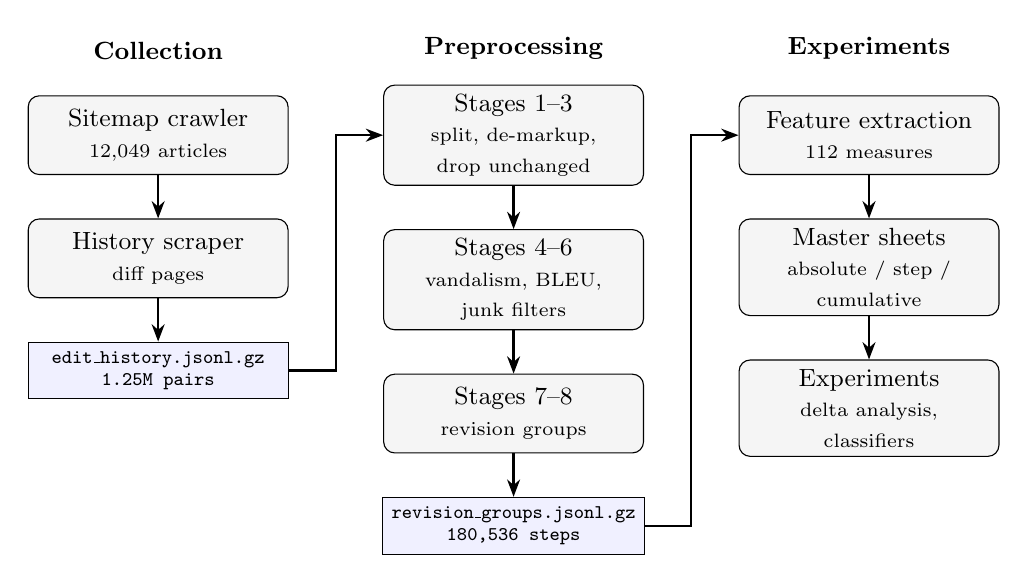
\begin{tikzpicture}[
  node distance=0.55cm and 0.5cm,
  box/.style={draw, rounded corners, align=center, minimum width=3.3cm, minimum height=1cm, font=\small, fill=gray!8},
  data/.style={draw, align=center, font=\scriptsize\ttfamily, fill=blue!6, minimum width=3.3cm},
  arr/.style={-{Stealth[length=2.2mm]}, thick}]
  \node[box] (crawl) {Sitemap crawler\\ \scriptsize 12{,}049 articles};
  \node[box, below=of crawl] (hist) {History scraper\\ \scriptsize diff pages};
  \node[data, below=of hist] (raw) {edit\_history.jsonl.gz\\ 1.25M pairs};
  \node[box, right=1.2cm of crawl] (clean) {Stages 1--3\\ \scriptsize split, de-markup,\\ \scriptsize drop unchanged};
  \node[box, below=of clean] (filter) {Stages 4--6\\ \scriptsize vandalism, BLEU,\\ \scriptsize junk filters};
  \node[box, below=of filter] (group) {Stages 7--8\\ \scriptsize revision groups};
  \node[data, below=of group] (rg) {revision\_groups.jsonl.gz\\ 180{,}536 steps};
  \node[box, right=1.2cm of clean] (feat) {Feature extraction\\ \scriptsize 112 measures};
  \node[box, below=of feat] (sheet) {Master sheets\\ \scriptsize absolute / step /\\ \scriptsize cumulative};
  \node[box, below=of sheet] (exp) {Experiments\\ \scriptsize delta analysis,\\ \scriptsize classifiers};
  \draw[arr] (crawl) -- (hist);
  \draw[arr] (hist) -- (raw);
  \draw[arr] (raw.east) -| ([xshift=-0.6cm]clean.west) -- (clean.west);
  \draw[arr] (clean) -- (filter);
  \draw[arr] (filter) -- (group);
  \draw[arr] (group) -- (rg);
  \draw[arr] (rg.east) -| ([xshift=-0.6cm]feat.west) -- (feat.west);
  \draw[arr] (feat) -- (sheet);
  \draw[arr] (sheet) -- (exp);
  \coordinate (hdr) at ([yshift=0.2cm]clean.north);
  \node[anchor=south, font=\small\bfseries] at (crawl.north |- hdr) {Collection};
  \node[anchor=south, font=\small\bfseries] at (clean.north |- hdr) {Preprocessing};
  \node[anchor=south, font=\small\bfseries] at (feat.north |- hdr) {Experiments};
\end{tikzpicture}
\caption{Overview of the three-stage pipeline used in this thesis.}
\label{fig:pipeline}
\end{figure}

\section{Data Collection}
\subsection{Building the Article Catalogue}
The wikiHow sitemap page lists every top-level category and its subcategories. A crawler written with \texttt{requests} and \texttt{BeautifulSoup} walked the sitemap from categories to subcategories to article links. It produced a catalogue of 12{,}049 articles in 20 categories and 372 subcategories. Table~\ref{tab:categories} shows how these articles are spread across categories. \emph{Relationships} is the largest category with 1{,}672 articles, followed by \emph{Education and Communications}, \emph{Health} and \emph{Computers and Electronics}, each with close to a thousand. The smallest categories contribute a few hundred articles each. The corpus therefore spans most areas of everyday life. (The site's own ``WikiHow'' category lists no articles.)

\begin{table}[ht]
\centering
\small
\caption{Articles per top-level category in the wikiHow sitemap catalogue.}
\label{tab:categories}
\begin{tabular}{@{}lrr@{}}
\toprule
Category & Subcategories & Articles\\
\midrule
Relationships & 12 & 1{,}672\\
Education and Communications & 28 & 1{,}076\\
Health & 41 & 987\\
Computers and Electronics & 26 & 960\\
Personal Care and Style & 24 & 892\\
Philosophy and Religion & 7 & 838\\
Hobbies and Crafts & 19 & 773\\
Home and Garden & 20 & 693\\
Arts and Entertainment & 17 & 646\\
Holidays and Traditions & 20 & 529\\
Food and Entertaining & 15 & 466\\
Pets and Animals & 31 & 463\\
Youth & 13 & 388\\
Cars \& Other Vehicles & 16 & 348\\
Finance and Business & 14 & 317\\
Family Life & 12 & 275\\
Work World & 22 & 269\\
Sports and Fitness & 14 & 262\\
Travel & 21 & 195\\
WikiHow & 0 & 0\\
\midrule
Total (20 categories) & 372 & 12{,}049\\
\bottomrule
\end{tabular}
\end{table}

\subsection{Scraping Edit Histories}
For each catalogued article, a second script visited the article's revision history for edits made between 2005 and 2026. It opened every comparison page that wikiHow shows between two consecutive revisions. On such a page, wikiHow aligns the old and new wikitext line by line and marks the changed lines. The scraper recorded each changed line as a \emph{base}/\emph{revised} pair, together with the URL of the comparison, which identifies the revision and its timestamp. Because a wikiHow step is usually written as one line of wikitext, a pair normally corresponds to one paragraph.

The scraper used a single persistent HTTP session, added randomised delays between requests and saved a checkpoint after each article, so that an interrupted run could resume without repeating work. Histories were retrieved for 7{,}955 of the 12{,}049 catalogued articles (66.0\%). The remaining articles could not be retrieved during the collection period; possible reasons include redirects, removed pages and history pages that require a logged-in session. The collected histories contain 1{,}247{,}332 base/revised pairs, a mean of 156.8 and a median of 88 pairs per article. All per-article files were bundled into one gzip-compressed JSON-lines file, with one article per line.

\section{Preprocessing Pipeline}
Raw edit pairs are noisy. They contain wiki markup, edits that only change formatting, vandalism and its reversal, and edits that replace a paragraph with unrelated text. The preprocessing stage removes these in eight numbered stages. Each filtering stage writes the surviving pairs to one folder and the discarded pairs to another, so every decision can be inspected.

\paragraph{Stage 1: Split.} The bundle is split into one JSON file per article.

\paragraph{Stage 2: Markup cleaning.} A modular cleaner removes wiki markup one type at a time i.e HTML comments, reference blocks, magic words, image/file/category links, templates, bold and italic quotes, header markers, list markers and any other HTML entities. Internal links are reduced to their visible text. Spacing around punctuation which is often damaged in the scraped text is then repaired. Pairs that become empty on both sides are dropped.

\paragraph{Stage 3: Unchanged pairs.} After cleaning, many pairs turn out to have identical text on both sides because the edit only touched markup. Both sides are compared using a normalised key i.e. whitespace collapsed, punctuation spacing fixed or case folded and pairs with identical keys are discarded.

\paragraph{Stage 4: Vandalism and revert cycles.} Vandalism on wikis is usually reverted quickly leaving a cycle in which text $A$ becomes $B$ and then returns to $A$. Within each article, edits are chained from oldest to newest using a whitespace insensitive, lower-cased key. If an earlier text reappears within five steps ($A\to B\to A$ or $A\to B\to C\to A$), every edge of that cycle is discarded then. Because vandals often change several lines in one revision, the filter then removes \emph{all} pairs that belong to the same revision as a discarded edge, together with any intermediate revisions between the vandal edit and its restoration.

\paragraph{Stage 5: Low-similarity pairs.} Some pairs are not revisions of the same paragraph but replacements by unrelated text, caused for example by misaligned lines in the comparison view. Similarity is measured with sentence-level BLEU \citep{papineni2002} between base and revision, computed in lower case with the smoothing method of \citet{chen2014}. Pairs with $\mathrm{BLEU} \le 0.06$ are discarded. The threshold was chosen by manual inspection of pairs near the boundary. Below it, pairs were almost always unrelated texts.

\paragraph{Stage 6: Junk.} Regular expressions remove pairs whose text is dominated by URLs, affiliated link query strings, leftover HTML tags, or the field names of quiz and JSON structures that wikiHow embeds in some of their articles. Arrow symbols such as ``$>$'' and ``$\rightarrow$'' are kept deliberately, because instructional text often uses them in menu paths (``File $>$ Save'').

\paragraph{Stage 7: Revision groups.} The surviving pairs are linked into chains. Starting from the oldest edit, a pair whose base matches the latest version of an existing chain (under the same normalised key) extends that chain. When several unused edges compete for the same base then the chronologically next one is taken and the others start chains of their own rather than being dropped. Each resulting chain is a \emph{revision group}: an ordered list of versions $v_0, v_1, \ldots, v_K$ of one paragraph, where $v_0$ is the original and $K$ is the \emph{depth} of the group.

\paragraph{Stage 8: Bundle.} All revision groups are written to a single JSON-lines file that is handed to the experiment stage.

Table~\ref{tab:funnel} shows how many pairs and articles remain after each stage. The filters are strict at the level of pairs: only 14.5\% of the raw pairs survive. Nearly half of the raw pairs (48\%) disappear at Stage~3, which shows how many logged edits change only markup or formatting. The vandalism filter then removes a further 45\% of what remains. This large share reflects both the amount of vandalism on an open wiki and the deliberately conservative design of the filter which discards every line of a suspicious revision. Articles, in contrast, are rarely lost, because an article is dropped only when none of its pairs survive.

\begin{table}[ht]
\centering
\small
\caption[Pairs and articles remaining after each preprocessing stage]{Edit pairs and articles remaining after each preprocessing stage. ``Kept'' is the share of the previous stage's pairs that survive.}
\label{tab:funnel}
\begin{tabular}{@{}llrrr@{}}
\toprule
Stage & Operation & Pairs & Kept (\%) & Articles\\
\midrule
1 & Split bundle into articles & 1{,}247{,}332 & -- & 7{,}955\\
2 & Markup cleaning & 1{,}162{,}667 & 93.2 & 7{,}862\\
3 & Remove unchanged pairs & 606{,}978 & 52.2 & 7{,}669\\
4 & Remove vandalism / revert cycles & 336{,}586 & 55.5 & 7{,}633\\
5 & Remove pairs with BLEU $\le 0.06$ & 188{,}539 & 56.0 & 7{,}548\\
6 & Remove junk pairs & 180{,}536 & 95.8 & 7{,}519\\
7--8 & Build and bundle revision groups & 180{,}536 & 100.0 & 7{,}519\\
\bottomrule
\end{tabular}
\end{table}

\section{The Final Corpus}
\subsection{Paragraph Level}
The final paragraph corpus contains 7{,}519 articles, 135{,}026 revision groups and 180{,}536 edit steps (one step for every consecutive pair $v_{k-1}\to v_k$). The distribution of depth is very skewed (Table~\ref{tab:depth}). About 78\% of all groups were revised only once, while a small tail of paragraphs was revised ten times or more, up to a maximum depth of 28.

\begin{table}[ht]
\centering
\small
\caption[Edit steps by revision depth]{Number of edit steps available at each revision depth $k$ (paragraph and sentence level). The step at depth $k$ exists only for groups of depth at least $k$.}
\label{tab:depth}
\begin{tabular}{@{}lrr@{}}
\toprule
Depth $k$ & Paragraph steps & Sentence steps\\
\midrule
1 & 135{,}026 & 163{,}466\\
2 & 29{,}627 & 21{,}973\\
3 & 8{,}939 & 4{,}219\\
4 & 3{,}510 & 1{,}122\\
5 & 1{,}594 & 348\\
6 & 791 & 131\\
7--10 & 887 & 96\\
$>$10 & 162 & 4\\
\midrule
Total & 180{,}536 & 191{,}359\\
\bottomrule
\end{tabular}
\end{table}

\subsection{Sentence Level}
A paragraph edit often changes only one of several sentences. To study edits at a finer grain, a sentence-level corpus was derived from the paragraph groups. Every version was split into sentences with the parser of the \texttt{en\_core\_web\_trf} spaCy pipeline \citep{honnibal2020}. For each paragraph step $v_{k-1}\to v_k$, the two sentence lists were aligned with a longest-matching-block algorithm:
\begin{itemize}
  \item sentences equal under the normalised key are \emph{unchanged} and are not counted as edits;
  \item within each block of replaced sentences, sentences are paired greedily by highest BLEU, each sentence used at most once, which covers one-to-one rewrites as well as splits and merges;
  \item inserted, deleted or unpaired sentences are recorded as additions or removals, not as edits.
\end{itemize}
Edits were then chained into sentence revision groups, in the same way as paragraphs. For each sentence, the text before it (\emph{prior}) and after it (\emph{post}) in the same paragraph version was kept as context. This alignment produced 208{,}508 sentence edit pairs (133{,}582 one-to-one and 74{,}926 from many-to-many blocks) in 176{,}271 groups. It also recorded 37{,}838 added and 18{,}948 removed sentences. As a final step, each group was split wherever the BLEU between consecutive versions was $\le 0.06$, the same threshold used for paragraphs, so that no comparison crosses a link between unrelated sentences. After this split, 191{,}359 sentence edit steps remain (Table~\ref{tab:depth}).

\section{Feature Extraction}
\label{sec:features}
Every version of every paragraph and sentence was described by 112 numeric measures. To keep the measures consistent, all of them use the same spaCy pipeline \texttt{en\_core\_web\_trf}, which is built on a transformer model, for sentence boundaries, POS tags and dependency trees. Paragraph-level values are computed sentence by sentence and then averaged with equal weight per sentence. This keeps a single long sentence from dominating the paragraph value.

\subsection{Surprisal with GPT-2}
GPT-2 small \citep{radford2019} was used to assign each subword token $t_i$ a surprisal of $-\log_2 P(t_i \mid t_{<i})$. At paragraph level, the whole paragraph is passed through the model in a single pass of up to 1{,}024 tokens, so that tokens in later sentences are conditioned on earlier sentences. Each token is then assigned to the sentence in which it starts. A sentence's mean surprisal is the average over its tokens, and the paragraph value \feat{mean_surprisal} is the mean over sentences:
\begin{equation}
  \bar S_{\text{para}} = \frac{1}{|\mathcal{S}|} \sum_{s \in \mathcal{S}} \frac{1}{|s|} \sum_{t_i \in s} -\log_2 P(t_i \mid t_{<i}).
\end{equation}
At sentence level, each sentence is scored on its own, and GPT-2's \texttt{<|endoftext|>} token is placed in front so that the first word also receives a surprisal value.

\subsection{Surprisal with $n$-gram Models}
To test whether the choice of language model matters (RQ2), twenty further surprisal measures were computed with $n$-gram models trained in SRILM \citep{stolcke2002}. Models of order $n \in \{1,\ldots,5\}$ were trained on four reference corpora of different style:
\begin{itemize}
  \item the \textbf{Brown} corpus \citep{francis1979}, a balanced corpus of 1960s American English;
  \item the \textbf{Wall Street Journal} section of the Penn Treebank \citep{marcus1993}, which contains newswire;
  \item \textbf{WikiText-2} \citep{merity2017}, which contains encyclopaedic Wikipedia text;
  \item \textbf{Simple English Wikipedia}, which contains encyclopaedic text written in simplified language.
\end{itemize}
Each corpus was lower-cased and tokenised into words, with one sentence per line. Unknown words were mapped to an \texttt{<unk>} class. At scoring time, each sentence of a paragraph was written on its own line with its own sentence boundary markers. SRILM's base-10 log probability was converted to bits and divided by the number of scored tokens. The resulting measures are named \nolinkurl{mean_surprisal_<corpus>_<n>}.

\subsection{Mean Dependency Length}
MDL follows eqn.~\eqref{eq:mdl}, with two adjustments for punctuation. Punctuation tokens and the root are not counted as dependents. If a word's head is a punctuation token, the head is replaced by the nearest non-punctuation ancestor. Distances are counted in words, so punctuation between a head and its dependent does not add to the length. A sentence without any arc (for example the one-word step heading ``Steps'') has no defined MDL. The paragraph value \feat{mean_mdl} is the unweighted mean over sentences.

\subsection{Linguistic Profile Features}
The remaining 90 measures follow the feature families of \citet{kazmi2022} and give a broad linguistic profile of each text.
\begin{itemize}
  \item \textbf{Raw (2):} mean and standard deviation of sentence length in tokens.
  \item \textbf{Lexical (17):} TTR, Maas TTR, MSTTR (window 25), MATTR, MTLD, moving-average MTLD, vocd-D and Yule's $K$, each computed once over characters and once over lower-cased words without punctuation (16 measures), plus lexical density, which counts content words (any noun, proper noun, verb, adjective or adverb) relative to function words.
  \item \textbf{POS ratios (8):} adverb/noun, adverb/pronoun, adjective/verb, noun/verb, verb/pronoun, adverb/adjective, adjective/pronoun and noun/pronoun.
  \item \textbf{Syntactic (63):} mean dependency tree depth, Szmrecsanyi's ISC, the ratio of argument to adjunct relations, the relative frequency of each Universal Dependencies relation, and a set of directional head--dependent POS bigrams (for example \feat{depbig_VERB_SCONJ_before}, a subordinating conjunction that precedes its verbal head).
\end{itemize}
For reference, the main lexical measures are defined as follows. $V$ is the number of distinct types, $N$ the number of tokens and $V(m,N)$ the number of types that occur exactly $m$ times:
\begin{align}
  \mathrm{TTR} &= \frac{V}{N}, &
  \text{Maas } a^2 &= \frac{\log N - \log V}{(\log N)^2}, &
  K &= 10^4 \cdot \frac{\sum_m m^2 V(m,N) - N}{N^2}.
\end{align}

\section{From Revision Groups to Datasets}
\label{sec:sheets}
The scored versions were joined into three ``master sheets''. Each one corresponds to a different question about a revision group $v_0, \ldots, v_K$.

\paragraph{Step pairs.} Every consecutive pair $(v_{k-1}, v_k)$ for $k = 1, \ldots, K$. For each feature $f$, the delta is $\Delta^{\text{step}}_k f = f(v_k) - f(v_{k-1})$. This captures the effect of a single edit.

\paragraph{Cumulative pairs.} Every pair $(v_0, v_k)$, which compares each revision with the original: $\Delta^{\text{cum}}_k f = f(v_k) - f(v_0)$. This captures the total effect of all edits up to depth $k$. At depth~1 the step and cumulative pairs are identical.

\paragraph{Absolute rows.} For each step pair, two rows are emitted, each holding the raw (not differenced) feature values of one version. The older version is labelled \emph{base} and the newer one \emph{edit}. An intermediate version $v_k$ ($0 < k < K$) therefore appears twice, once as \emph{edit} of $v_{k-1}$ and once as \emph{base} of $v_{k+1}$. This sheet tests whether a version can be recognised as revised \emph{on its own}, without its partner.

Table~\ref{tab:example} illustrates the three sheets with one revision group from the article \emph{00s Music Quiz}.

\begin{table}[ht]
\centering
\small
\caption{A two-step revision group and the pairs it produces in each sheet.}
\label{tab:example}
\begin{tabularx}{\textwidth}{@{}lX@{}}
\toprule
Version & Text\\
\midrule
$v_0$ & For more information about\ldots\\
$v_1$ & For more information about 2000's music, check out these resources.\\
$v_2$ & For more information about 2000s music, check out these resources.\\
\midrule
Step & $(v_0, v_1)$, $(v_1, v_2)$\\
Cumulative & $(v_0, v_1)$, $(v_0, v_2)$\\
Absolute & $v_0$:\,base, $v_1$:\,edit, $v_1$:\,base, $v_2$:\,edit\\
\bottomrule
\end{tabularx}
\end{table}

\section{Handling Undefined Values and Feature Selection}
\label{sec:featsel}
For some measures a value of zero means that the measure \emph{could not be computed}, not that its true value is zero. Examples are the MDL of a one-word heading, the GPT-2 surprisal of a text with a single token, and vocd-D for texts with fewer than 36 tokens. Two rules were applied to such values. Any measure that was undefined in more than 5\% of rows was removed, which eliminated both vocd-D variants. Any version for which a retained measure was undefined was listed, and every pair that contains such a version was excluded from all experiments, so that undefined values never enter a model as if they were real zeros.

The 112 candidate features were then reduced in three further steps:
\begin{enumerate}
  \item \textbf{Constant features} that take a single value in every row were removed.
  \item \textbf{Highly correlated features}: for every pair with $|r| > 0.90$ one member was removed. When MDL was part of such a pair, MDL was kept, because it is one of the two theory-driven measures under study.
  \item \textbf{One surprisal measure}: after the correlation filter, GPT-2 surprisal and two $n$-gram surprisals remained. Only GPT-2 surprisal was kept. Experiment~II (Section~\ref{sec:exp1}) shows that it is the most informative surprisal measure, and keeping one measure makes its coefficient easier to interpret.
\end{enumerate}
This left 71 features at paragraph level. The same procedure was run separately on the sentence sheet and left 69 features: the paragraph set minus \feat{word_msttr} and \feat{word_yulek}, which the correlation filter removes at sentence level because in texts as short as one sentence, they move almost in step with the other word-level diversity measures. These sets are used in the full-feature models of Chapter~\ref{ch:exp2}.

\section{Modelling Set-up}
\label{sec:setup}
\subsection{Train/Test Split}
All classifiers use one fixed split \emph{by article}. A random 20\% of articles (1{,}504 of 7{,}519, seed 42) form the test set, and the rest form the training set. Splitting by article rather than by pair prevents a model from seeing one edit of a paragraph during training and a closely related edit of the same paragraph at test time. The same list of test articles is used at both paragraph and sentence level, so results at the two levels are measured on exactly the same articles.

\subsection{Randomised Pair Presentation}
For the step and cumulative sheets, each pair is shown to the model as $(A, B)$ in random order. With probability one half $A$ is the base and $B$ the revision (label 1), and otherwise the order is reversed (label 0). Every feature is entered as the difference $f(B) - f(A)$. Text features are represented by the difference of TF-IDF vectors, $\mathbf{x}_{\text{text}} = \text{tfidf}(B) - \text{tfidf}(A)$. As a result the classes are balanced by construction, chance accuracy is 50\%, and a model cannot exploit position.

\subsection{Models}
\paragraph{TF-IDF baseline.} Word unigrams and bigrams with a minimum document frequency of 2 and a vocabulary capped at 20{,}000 features, fitted on the training texts only.

\paragraph{Logistic regression.} L2-regularised logistic regression \citep{pedregosa2011} on TF-IDF features, on numeric features, or on both concatenated. Each numeric feature is rescaled to mean~0 and standard deviation~1, with the scaling learned from the training set only. Because all numeric inputs share a scale, the absolute value of a coefficient shows how strongly that feature pushes the decision.

\paragraph{Gradient-boosted trees.} The histogram variant of gradient boosting \citep{friedman2001}, with learning rate 0.1, up to 500 trees and early stopping on a 10\% validation slice. It is trained on the selected numeric features only (71 at paragraph level, 69 at sentence level), since trees are inefficient on 20{,}000 sparse text columns. Unlike logistic regression, trees can learn interactions between features.

\subsection{Evaluation}
Models are evaluated on held-out articles with accuracy, precision, recall, F1 (positive class: \emph{edit}) and AUC, which is the chance that a randomly drawn positive example receives a higher score than a randomly drawn negative one. On the absolute sheet, row-level accuracy is limited because intermediate versions appear with both labels. For this sheet a \emph{pair accuracy} is therefore also reported: a pair counts as correct when the model gives the revised version a higher score than its base.

%% =====================================================================
%%  CHAPTER 4 -- EXPERIMENT I
%% =====================================================================
\chapter{Experiment I: How Cognitive-Load Measures Change Across Revisions}
\label{ch:exp1}

The first experiment is descriptive and addresses RQ1 and RQ2. It does not train any model. It simply measures that for every edit in the corpus how surprisal and MDL changes and summarises these changes by direction, size and revision depth.

\section{Set-up}
Twenty-two measures were analysed: \feat{mean_mdl}, GPT-2 \feat{mean_surprisal}, and the twenty SRILM surprisal variants. For every revision group and every depth $k \ge 1$, both the step delta $\Delta^{\text{step}}_k$ and the cumulative delta $\Delta^{\text{cum}}_k$ were computed. Deltas were rounded to five decimal places. This is the precision of the stored feature values, so that floating point noise is not counted as a change. Each delta was then classified as positive (the measure went up), zero or negative (it went down). For each measure, delta type and depth, the analysis reports:
\begin{itemize}
  \item the percentage of positive, zero and negative deltas;
  \item the mean delta within the positive group and within the negative group;
  \item the net mean delta over all pairs and the median delta.
\end{itemize}
Because a measure can rise in many edits by a small amount while falling in fewer edits by a large amount, the sign proportions and the mean must be read together. The median is the most robust single summary of the typical edit.

\section{Results at Paragraph Level}
\subsection{Overall Direction of Change}
Table~\ref{tab:delta-para} summarises the deltas over all 180{,}536 paragraph edits.

\begin{table}[ht]
\centering
\small
\caption[Change in cognitive-load measures (paragraph level)]{Direction and size of change in cognitive-load measures across all paragraph edits ($n = 180{,}536$ per row). ``Up/Zero/Down'' give the percentage of edits in which the measure increased, did not change or decreased. Surprisal is in bits per token, MDL in words.}
\label{tab:delta-para}
\setlength{\tabcolsep}{4.5pt}
\begin{tabular}{@{}llrrrrr@{}}
\toprule
Measure & Delta & Up (\%) & Zero (\%) & Down (\%) & Mean $\Delta$ & Median $\Delta$\\
\midrule
\multirow{2}{*}{GPT-2 surprisal} & step & 44.3 & 0.0 & \textbf{55.7} & $+0.033$ & $\mathbf{-0.038}$\\
 & cumulative & 43.6 & 0.0 & \textbf{56.4} & $-0.005$ & $\mathbf{-0.053}$\\
\midrule
\multirow{2}{*}{MDL} & step & 40.6 & 23.6 & 35.8 & $+0.007$ & $0.000$\\
 & cumulative & 43.0 & 19.6 & 37.5 & $+0.011$ & $0.000$\\
\midrule
\multirow{2}{*}{WikiText-2, 1-gram} & step & 52.1 & 6.5 & 41.3 & $+0.067$ & $+0.009$\\
 & cumulative & 53.1 & 5.1 & 41.7 & $+0.073$ & $+0.016$\\
\multirow{2}{*}{Brown, 3-gram} & step & 48.4 & 6.3 & 45.3 & $+0.132$ & $0.000$\\
 & cumulative & 49.4 & 4.9 & 45.7 & $+0.133$ & $0.000$\\
\multirow{2}{*}{PTB-WSJ, 3-gram} & step & 48.3 & 6.7 & 45.1 & $+0.130$ & $0.000$\\
 & cumulative & 49.1 & 5.3 & 45.6 & $+0.130$ & $0.000$\\
\multirow{2}{*}{Simple Wiki, 3-gram} & step & 49.4 & 6.1 & 44.5 & $+0.108$ & $0.000$\\
 & cumulative & 50.1 & 4.8 & 45.1 & $+0.107$ & $+0.001$\\
\bottomrule
\end{tabular}
\end{table}

Three patterns stand out.

\paragraph{GPT-2 surprisal tends to fall.} In about 56\% of edits the revised paragraph is less surprising to GPT-2 than the version it replaced. The median change is negative for both step ($-0.038$ bits) and cumulative ($-0.053$ bits) deltas. Changes of exactly zero almost never occur since nearly any change to the words alters the model's probabilities. The mean behaves differently from the median. For step deltas the mean is slightly positive ($+0.033$) because increases, though less frequent, are larger on average ($+0.73$ bits against $-0.52$). The distribution therefore has a long right tail of a few large increases. This tail is consistent with edits that add new, specific content: a phrase such as ``2000s music'' that fills in an unfinished sentence makes the text more informative and therefore locally more surprising.

\paragraph{MDL does not fall.} For MDL a large share of edits (20--24\%) leaves the value unchanged. This is expected since many edits change words without changing sentence structure. Among the edits that do change MDL, increases are slightly more common than decreases (43.0\% against 37.5\% cumulatively) and both the mean ($+0.011$) and the median ($0$) shows no reduction. At the level of the whole corpus there is no evidence that revisers shorten dependencies.

\paragraph{$n$-gram surprisal tends to rise.} All $n$-gram measures move in the \emph{opposite} direction to GPT-2. Under the WikiText-2 unigram model, 52--53\% of edits \emph{increase} surprisal and the median is positive. Under the 3-gram models, increases are slightly more frequent than decreases and the mean rises by more than a tenth of a bit. The same pattern holds for every corpus and every order (the full set of 20 variants is in the output tables). Chapter~\ref{ch:discussion} discusses why two estimates of the same quantity disagree. In brief, $n$-gram models estimated from non wikiHow corpora assign high surprisal to the specific, content-rich vocabulary that revisions tend to add, while GPT-2 rewards the same additions for making the text more coherent in context.

\subsection{Change by Revision Depth}
Figure~\ref{fig:gpt2-depth} breaks the cumulative GPT-2 deltas down by revision depth, and Table~\ref{tab:depth-para} lists the numbers for the first ten depths.

\begin{figure}[!htbp]
\centering
\safefig{figures/para-gpt2-cumulative.png}{0.98\textwidth}
\caption[Cumulative change in GPT-2 surprisal by depth (paragraph level)]{Cumulative change in GPT-2 surprisal, $\Delta = S(v_k) - S(v_0)$, by revision depth $k$ for paragraphs. Red: mean among edits where surprisal rose. Blue: mean among edits where it fell. Black: net mean over all edits. Only depths with at least 50 pairs are shown.}
\label{fig:gpt2-depth}
\end{figure}

\begin{table}[ht]
\centering
\small
\caption[Cumulative change by revision depth (paragraph level)]{Cumulative change relative to the original paragraph, by revision depth. ``Down'' and ``Up'' give the share of pairs at that depth in which the measure decreased or increased.}
\label{tab:depth-para}
\begin{tabular}{@{}rrrrrr@{}}
\toprule
 & & \multicolumn{2}{c}{GPT-2 surprisal} & \multicolumn{2}{c}{MDL}\\
\cmidrule(lr){3-4}\cmidrule(lr){5-6}
Depth & Pairs & Net mean $\Delta$ & Down (\%) & Net mean $\Delta$ & Up (\%)\\
\midrule
1 & 135{,}026 & $+0.050$ & 55.1 & $+0.008$ & 40.5\\
2 & 29{,}627 & $-0.113$ & 59.5 & $+0.013$ & 49.0\\
3 & 8{,}939 & $-0.249$ & 62.1 & $+0.020$ & 52.4\\
4 & 3{,}510 & $-0.284$ & 62.2 & $+0.028$ & 52.5\\
5 & 1{,}594 & $-0.296$ & 61.6 & $+0.030$ & 53.3\\
6 & 791 & $-0.314$ & 62.3 & $+0.056$ & 56.9\\
7 & 413 & $-0.314$ & 62.7 & $+0.067$ & 57.9\\
8 & 244 & $-0.226$ & 57.8 & $+0.066$ & 57.4\\
9 & 135 & $-0.303$ & 60.7 & $+0.057$ & 57.8\\
10 & 95 & $-0.317$ & 61.1 & $+0.086$ & 56.8\\
\bottomrule
\end{tabular}
\end{table}

The depth profile sharpens the overall picture. At depth~1 the net mean is slightly positive but already 55\% of first edits lower surprisal. From depth~2 onward the net change is clearly negative and it grows to about $-0.25$ bits by depth~3. It then stays near $-0.3$ bits, with roughly 62\% of revised paragraphs less surprising than their originals. The mean among decreasing edits deepens steadily, from $-0.57$ at depth~1 to about $-0.80$ at depth~6, while the mean among increasing edits shrinks from $+0.81$ to about $+0.50$. In other words, as a paragraph is revised again and again, its distance from the original is increasingly made up of reductions in surprisal.

MDL shows the opposite drift (Figure~\ref{fig:mdl-depth}). The cumulative mean change in MDL is small but positive at every depth and grows with depth, and from depth~2 onward more than half of the revised paragraphs have \emph{longer} mean dependencies than their original. One plausible reason is that heavily revised paragraphs grow longer as contributors add clauses, conditions and examples, and more complex sentences tend to contain longer dependencies.

\begin{figure}[ht]
\centering
\safefig{figures/para-mdl-cumulative.png}{0.95\textwidth}
\caption[Cumulative change in MDL by depth (paragraph level)]{Cumulative change in mean dependency length by revision depth for paragraphs (same layout as Figure~\ref{fig:gpt2-depth}).}
\label{fig:mdl-depth}
\end{figure}

One caution applies when reading these trends. Groups that reach a high depth are not a random sample, since they are paragraphs that attracted repeated attention. The depth profile therefore mixes two effects: the cumulative effect of more edits, and whatever makes a paragraph likely to be edited many times. The analysis describes what happens to such paragraphs but cannot separate the two causes.

\section{Results at Sentence Level}
The same analysis was repeated on the 191{,}359 sentence edits (Table~\ref{tab:delta-sent} and Figure~\ref{fig:sent-gpt2}).

\begin{table}[ht]
\centering
\small
\caption[Change in cognitive-load measures (sentence level)]{Direction and size of change in cognitive-load measures across all sentence edits ($n = 191{,}359$ per row).}
\label{tab:delta-sent}
\setlength{\tabcolsep}{4.5pt}
\begin{tabular}{@{}llrrrrr@{}}
\toprule
Measure & Delta & Up (\%) & Zero (\%) & Down (\%) & Mean $\Delta$ & Median $\Delta$\\
\midrule
\multirow{2}{*}{GPT-2 surprisal} & step & 44.2 & 0.0 & \textbf{55.8} & $\mathbf{-0.026}$ & $\mathbf{-0.083}$\\
 & cumulative & 43.7 & 0.2 & \textbf{56.0} & $\mathbf{-0.046}$ & $\mathbf{-0.093}$\\
\midrule
\multirow{2}{*}{MDL} & step & 38.0 & 29.4 & 32.6 & $+0.020$ & $0.000$\\
 & cumulative & 39.5 & 27.3 & 33.2 & $+0.027$ & $0.000$\\
\midrule
\multirow{2}{*}{WikiText-2, 1-gram} & step & 51.3 & 8.2 & 40.6 & $+0.080$ & $+0.013$\\
 & cumulative & 51.9 & 7.5 & 40.6 & $+0.089$ & $+0.019$\\
\multirow{2}{*}{Brown, 3-gram} & step & 47.4 & 7.8 & 44.8 & $+0.122$ & $0.000$\\
 & cumulative & 48.1 & 7.1 & 44.8 & $+0.130$ & $0.000$\\
\bottomrule
\end{tabular}
\end{table}

\begin{figure}[ht]
\centering
\safefig{figures/sent-gpt2-cumulative.png}{0.95\textwidth}
\caption[Cumulative change in GPT-2 surprisal by depth (sentence level)]{Cumulative change in GPT-2 surprisal by revision depth for sentences.}
\label{fig:sent-gpt2}
\end{figure}

At sentence level the reduction in GPT-2 surprisal is clearer than at paragraph level. Both the mean and the median are negative for step and cumulative deltas, and the median reduction ($-0.08$ to $-0.09$ bits) is more than twice the paragraph value. The cumulative net change becomes more negative with depth: $-0.025$ at depth~1, $-0.132$ at depth~2, $-0.277$ at depth~3 and $-0.359$ at depth~4. The likely reason is that a sentence edit isolates the part of the paragraph that has actually changed whereas a paragraph average dilutes that change with sentences that were left untouched. MDL and the $n$-gram measures behave as they do at paragraph level: MDL does not fall, and the $n$-gram surprisals rise.

\section{Summary of Experiment I}
\begin{itemize}
  \item \textbf{RQ1, surprisal.} Revisions typically make text less surprising to a contextual language model. About 56\% of edits reduce GPT-2 surprisal at both levels, the median change is always negative, and the cumulative reduction grows with the number of revisions.
  \item \textbf{RQ1, dependency length.} There is no corpus-wide reduction in MDL. Between a fifth and a third of edits leave it unchanged, and among those that do change it, increases slightly outnumber decreases.
  \item \textbf{RQ2.} Whether surprisal appears to fall or rise is decided by the language model used to measure it. $n$-gram models trained on Brown, PTB-WSJ, WikiText-2 or Simple Wikipedia report a slight \emph{increase} in surprisal for the same edits.
\end{itemize}

%% =====================================================================
%%  CHAPTER 5 -- EXPERIMENT II
%% =====================================================================
\chapter{Experiment II: Distinguishing Original from Revised Text}
\label{ch:exp2}

Experiment~I showed that surprisal changes in a consistent direction on average. Experiment~II asks whether this regularity is strong enough to be \emph{useful}: given two versions of a paragraph, can a model tell which one is the revision and how much do surprisal and MDL contribute? Five sub experiments build on one another. All use the article-level split, randomised pair order and metrics described in Section~\ref{sec:setup}.

\section{Experiment II-1: Which Surprisal Measure Is Most Useful?}
\label{sec:exp1}
\subsection{Design}
A logistic regression was trained on TF-IDF features plus \emph{one} surprisal measure at a time, for each of the 21 measures (GPT-2 and the 20 $n$-gram variants), on all three sheets. A TF-IDF-only model serves as the baseline.

\subsection{Results}
Table~\ref{tab:exp1} reports test accuracy for every variant.

\begin{table}[ht]
\centering
\small
\caption[Experiment II-1: TF-IDF plus one surprisal measure]{Experiment II-1: test accuracy of logistic regression with TF-IDF plus one surprisal measure (paragraph level). The best $n$-gram order per corpus is underlined.}
\label{tab:exp1}
\begin{tabular}{@{}llccc@{}}
\toprule
Surprisal source & Order & Absolute & Cumulative & Step\\
\midrule
\multicolumn{2}{@{}l}{TF-IDF only (baseline)} & 0.5446 & 0.6437 & 0.6205\\
\multicolumn{2}{@{}l}{\textbf{+ GPT-2}} & 0.5448 & \textbf{0.6828} & \textbf{0.6637}\\
\midrule
\multirow{5}{*}{+ Brown} & 1 & 0.5449 & 0.6401 & 0.6164\\
 & 2 & 0.5443 & 0.6557 & 0.6295\\
 & 3 & 0.5441 & 0.6559 & 0.6295\\
 & 4 & 0.5444 & \underline{0.6578} & \underline{0.6322}\\
 & 5 & 0.5447 & 0.6567 & 0.6317\\
\midrule
\multirow{5}{*}{+ PTB-WSJ} & 1 & 0.5450 & 0.6434 & 0.6139\\
 & 2 & 0.5449 & 0.6535 & 0.6267\\
 & 3 & 0.5448 & 0.6547 & 0.6282\\
 & 4 & 0.5449 & \underline{0.6556} & \underline{0.6302}\\
 & 5 & 0.5451 & 0.6545 & 0.6297\\
\midrule
\multirow{5}{*}{+ WikiText-2} & 1 & 0.5460 & \underline{0.6544} & \underline{0.6304}\\
 & 2 & 0.5453 & 0.6474 & 0.6198\\
 & 3 & 0.5456 & 0.6484 & 0.6187\\
 & 4 & 0.5462 & 0.6481 & 0.6207\\
 & 5 & 0.5458 & 0.6491 & 0.6220\\
\midrule
\multirow{5}{*}{+ Simple Wiki} & 1 & 0.5453 & \underline{0.6516} & 0.6228\\
 & 2 & 0.5446 & 0.6472 & 0.6214\\
 & 3 & 0.5444 & 0.6462 & 0.6225\\
 & 4 & 0.5447 & 0.6469 & 0.6210\\
 & 5 & 0.5446 & 0.6476 & \underline{0.6245}\\
\bottomrule
\end{tabular}
\end{table}

On both pair sheets GPT-2 surprisal is clearly the most useful single addition. It raises cumulative accuracy by 3.9 points (from 64.4\% to 68.3\%) and step accuracy by 4.3 points (from 62.1\% to 66.4\%). The best $n$-gram variant, Brown 4-gram, adds only 1.4 and 1.2 points. Among the $n$-gram models, those trained on the general Brown corpus and on newswire work better at higher orders, while for WikiText-2 the unigram model is the best. No $n$-gram variant comes close to GPT-2.

On the absolute sheet, all variants score between 54.4\% and 54.6\%, barely above chance and indistinguishable from the baseline. Judging a single version on its own, without its partner, is much harder. The rest of this chapter therefore concentrates on the pair sheets.

The same comparison on the sentence sheet gives the same ranking with wider margins. GPT-2 surprisal raises cumulative accuracy from 60.5\% to 66.0\% ($+5.6$ points) and step accuracy from 59.7\% to 65.4\% ($+5.7$ points). The best $n$-gram variant at sentence level is the WikiText-2 unigram model, which adds only 1.6 and 1.7 points (62.0\% and 61.4\%). Higher-order Brown and PTB-WSJ models add between 1.2 and 1.6 points, so no $n$-gram variant reaches more than about a third of the GPT-2 gain. On the absolute sheet all sentence variants again lie between 54.6\% and 55.3\%.

These results support the choice of GPT-2 surprisal as the representative surprisal feature for the remaining experiments.

\section{Experiment II-2: Surprisal versus Dependency Length}
\subsection{Design}
Four feature sets were compared: TF-IDF alone, TF-IDF + GPT-2 surprisal, TF-IDF + MDL, and TF-IDF + both. Precision, recall and F1 are reported in addition to accuracy and AUC.

\subsection{Results}
\begin{table}[ht]
\centering
\small
\caption[Experiment II-2: surprisal and MDL over TF-IDF]{Experiment II-2: contribution of surprisal and MDL on top of TF-IDF (paragraph level, logistic regression). Absolute-sheet results are row-level.}
\label{tab:exp2}
\begin{tabular}{@{}llccccc@{}}
\toprule
Sheet & Feature set & Acc. & Prec. & Rec. & F1 & AUC\\
\midrule
\multirow{4}{*}{Cumulative} & TF-IDF & 0.6437 & 0.6671 & 0.5755 & 0.6179 & 0.7178\\
 & + surprisal & 0.6828 & 0.6854 & 0.6773 & 0.6813 & 0.7436\\
 & + MDL & 0.6443 & 0.6666 & 0.5792 & 0.6198 & 0.7179\\
 & + both & \textbf{0.6834} & \textbf{0.6865} & 0.6763 & \textbf{0.6814} & \textbf{0.7442}\\
\midrule
\multirow{4}{*}{Step} & TF-IDF & 0.6205 & 0.6515 & 0.5249 & 0.5814 & 0.6850\\
 & + surprisal & \textbf{0.6637} & \textbf{0.6728} & \textbf{0.6428} & \textbf{0.6575} & 0.7161\\
 & + MDL & 0.6199 & 0.6509 & 0.5240 & 0.5806 & 0.6855\\
 & + both & 0.6634 & 0.6727 & 0.6421 & 0.6570 & \textbf{0.7166}\\
\midrule
\multirow{4}{*}{Absolute} & TF-IDF & 0.5446 & 0.5401 & 0.6007 & 0.5688 & 0.5757\\
 & + surprisal & 0.5448 & 0.5398 & 0.6083 & 0.5720 & 0.5755\\
 & + MDL & 0.5450 & 0.5397 & 0.6110 & 0.5732 & 0.5760\\
 & + both & 0.5450 & 0.5400 & 0.6064 & 0.5713 & 0.5757\\
\bottomrule
\end{tabular}
\end{table}

Table~\ref{tab:exp2} gives a clear answer. Adding surprisal improves every metric on both pair sheets. Most of the gain comes from recall, which rises from 0.58 to 0.68 on cumulative pairs. On its own, the TF-IDF model is conservative: when the two versions differ only slightly in wording, it often fails to recognise which one is the revision. Surprisal supplies evidence that words alone do not, and lets the model identify many of these revisions. Adding MDL changes accuracy by less than 0.1 points in every setting, both with and without surprisal. Taken together with Experiment~I, this suggests that dependency length carries almost no information about the direction of an edit in this data.

\section{Experiment II-3: The Full Linguistic Profile}
\subsection{Design}
Two logistic regressions were trained with the selected features (Section~\ref{sec:featsel}): one on the features alone and one on TF-IDF plus the features. The experiment was run at both levels, with 71 features on the paragraph sheets and 69 on the sentence sheets. On the absolute sheet, pair accuracy is reported (revision scored above base).

\subsection{Results}
\begin{table}[ht]
\centering
\small
\caption[Experiment II-3: logistic regression with 71 features]{Experiment II-3: logistic regression with the 71 selected features (paragraph level). Absolute accuracy is pair accuracy; the other absolute metrics are row-level.}
\label{tab:exp3}
\begin{tabular}{@{}llccccc@{}}
\toprule
Sheet & Feature set & Acc. & Prec. & Rec. & F1 & AUC\\
\midrule
\multirow{2}{*}{Cumulative} & 71 features & 0.6791 & 0.6840 & 0.6669 & 0.6754 & 0.7328\\
 & TF-IDF + 71 & \textbf{0.6944} & \textbf{0.6968} & \textbf{0.6897} & \textbf{0.6932} & \textbf{0.7578}\\
\midrule
\multirow{2}{*}{Step} & 71 features & 0.6600 & 0.6680 & 0.6419 & 0.6547 & 0.7043\\
 & TF-IDF + 71 & \textbf{0.6740} & \textbf{0.6809} & \textbf{0.6601} & \textbf{0.6703} & \textbf{0.7293}\\
\midrule
\multirow{2}{*}{Absolute} & 71 features & 0.5791 & 0.5366 & 0.6141 & 0.5727 & 0.5706\\
 & TF-IDF + 71 & \textbf{0.6052} & 0.5458 & 0.5961 & 0.5699 & \textbf{0.5864}\\
\bottomrule
\end{tabular}
\end{table}

Even without any word features, the 71 linguistic measures reach 67.9\% accuracy on cumulative pairs, slightly below TF-IDF + surprisal (68.3\%). Combining them with TF-IDF gives the best linear model: 69.4\% accuracy and 0.758 AUC on cumulative pairs, and 67.4\% accuracy on step pairs (Table~\ref{tab:exp3}). Scoring the absolute sheet by pairs raises its accuracy from about 54.5\% to 60.5\%, which confirms that row-level scores on that sheet understate what the model has learned.

\begin{table}[ht]
\centering
\small
\caption[Experiment II-3: logistic regression with 69 features (sentence level)]{Experiment II-3 at sentence level: logistic regression with the 69 selected features. Absolute accuracy is pair accuracy; the other absolute metrics are row-level.}
\label{tab:exp3-sent}
\begin{tabular}{@{}llccccc@{}}
\toprule
Sheet & Feature set & Acc. & Prec. & Rec. & F1 & AUC\\
\midrule
\multirow{2}{*}{Cumulative} & 69 features & 0.6447 & 0.6500 & 0.6312 & 0.6404 & 0.6953\\
 & TF-IDF + 69 & \textbf{0.6662} & \textbf{0.6705} & \textbf{0.6570} & \textbf{0.6636} & \textbf{0.7279}\\
\midrule
\multirow{2}{*}{Step} & 69 features & 0.6379 & 0.6424 & 0.6275 & 0.6349 & 0.6834\\
 & TF-IDF + 69 & \textbf{0.6599} & \textbf{0.6630} & \textbf{0.6549} & \textbf{0.6589} & \textbf{0.7181}\\
\midrule
\multirow{2}{*}{Absolute} & 69 features & 0.5894 & 0.5386 & 0.6059 & 0.5703 & 0.5696\\
 & TF-IDF + 69 & \textbf{0.6167} & 0.5542 & 0.5934 & 0.5731 & \textbf{0.5929}\\
\bottomrule
\end{tabular}
\end{table}

The sentence-level results (Table~\ref{tab:exp3-sent}) follow the same pattern at a lower level. The 69 measures alone reach 64.5\% on cumulative and 63.8\% on step pairs, already above TF-IDF alone at that level (60.5\% and 59.7\%). Adding TF-IDF gives 66.6\% and 66.0\%, only about half a point above TF-IDF + surprisal (66.0\% and 65.4\%). At sentence level, therefore, almost all of what the full profile adds to the word features is already carried by surprisal. On the absolute sheet, pair accuracy rises to 61.7\%, slightly higher than at paragraph level.

\subsection{Which Features Matter?}
Because all numeric features were standardised, their coefficients in the TF-IDF + 71 model can be compared directly. Table~\ref{tab:weights} lists the ten largest by mean absolute weight over the cumulative and step models. A negative weight means that a \emph{decrease} in the feature from $A$ to $B$ makes the model more confident that $B$ is the revision.

\begin{table}[ht]
\centering
\small
\caption[Most influential features in the full linear model]{Ten most influential features in the TF-IDF + 71-feature logistic regression (standardised coefficients). Negative = a lower value points to the revised version.}
\label{tab:weights}
\begin{tabular}{@{}lrrl@{}}
\toprule
Feature & Cumulative & Step & Interpretation\\
\midrule
\feat{ttr} (character) & $-0.590$ & $-0.430$ & lexical diversity\\
\feat{mean_surprisal} (GPT-2) & $-0.424$ & $-0.367$ & predictability\\
\feat{maas_ttr} (character) & $-0.335$ & $-0.248$ & length-corrected diversity\\
\feat{dep_aux} & $-0.265$ & $-0.221$ & auxiliary verbs\\
\feat{word_ttr} & $-0.202$ & $-0.145$ & word-level diversity\\
\feat{depbig_VERB_SCONJ_before} & $-0.199$ & $-0.166$ & preposed subordinators\\
\feat{dep_advmod} & $-0.169$ & $-0.139$ & adverbial modifiers\\
\feat{mean_mdl} & $-0.165$ & $-0.137$ & dependency length\\
\feat{depbig_VERB_PRON_before} & $-0.124$ & $-0.103$ & preverbal pronouns\\
\feat{std_sen_len} & $+0.087$ & $+0.077$ & sentence-length variation\\
\bottomrule
\end{tabular}
\end{table}

Three observations follow from this table. First, GPT-2 surprisal remains the second strongest feature even when 70 other measures are available, so its information is not duplicated by the lexical and syntactic profile. Second, the strongest feature is character-level TTR, together with two other diversity measures. A lower TTR in the revision partly reflects the fact that revised paragraphs are often longer, and TTR falls with length. It also matches the reduction in surprisal, since text that reuses its own vocabulary is easier to predict. Third, MDL has a \emph{negative} weight once the other features are held constant, even though it added nothing on its own in Experiment~II-2. This suggests that a reduction in dependency length may still be present for edits of a given length and structure, but is hidden in the raw deltas because revisions also tend to make sentences longer and more complex.

The same model at sentence level partly confirms this picture. GPT-2 surprisal becomes the single strongest feature, with weights of $-0.549$ (cumulative) and $-0.520$ (step), ahead of character TTR ($-0.347$, $-0.293$) and Maas TTR ($-0.242$, $-0.197$). The preposed-subordinator, adverbial-modifier and auxiliary features again follow with negative weights. Two differences stand out. First, \feat{word_ttr} changes sign and takes a small positive weight ($+0.093$, $+0.095$). Second, the negative MDL weight seen at paragraph level does not reappear and at sentence level \feat{mean_mdl} it has a weight close to zero ($+0.030$, $+0.017$) and ranks only 23rd. The conditional MDL effect found for paragraphs should therefore be read with caution, since it does not hold within single sentences.

\section{Experiment II-4: A Non-linear Model}
\subsection{Design}
A logistic regression treats each feature as an independent additive effect. The tree model was used to test whether interactions between features (for example, ``a drop in TTR matters only when surprisal also falls'') improve prediction. Gradient-boosted trees were trained on the selected features alone (71 at paragraph level, 69 at sentence level).

\subsection{Results}
\begin{table}[ht]
\centering
\small
\caption[Experiment II-4: gradient-boosted trees]{Experiment II-4: gradient-boosted trees on the selected features (71 at paragraph level, 69 at sentence level). ``Trees'' is the number of boosting rounds chosen by early stopping.}
\label{tab:exp4}
\begin{tabular}{@{}llcccccr@{}}
\toprule
Level & Sheet & Acc. & Prec. & Rec. & F1 & AUC & Trees\\
\midrule
\multirow{4}{*}{Paragraph} & Cumulative & \textbf{0.7081} & 0.7120 & 0.6999 & 0.7059 & \textbf{0.7824} & 257\\
 & Step & \textbf{0.6921} & 0.6940 & 0.6919 & 0.6929 & \textbf{0.7658} & 169\\
 & Absolute (rows) & 0.5557 & 0.5444 & 0.6831 & 0.6059 & 0.5907 & 47\\
 & Absolute (pairs) & 0.5647 & -- & -- & -- & -- & --\\
\midrule
\multirow{4}{*}{Sentence} & Cumulative & 0.6752 & 0.6782 & 0.6699 & 0.6740 & 0.7505 & 292\\
 & Step & 0.6653 & 0.6691 & 0.6583 & 0.6637 & 0.7437 & 222\\
 & Absolute (rows) & 0.5618 & 0.5542 & 0.6323 & 0.5907 & 0.5974 & 48\\
 & Absolute (pairs) & 0.5975 & -- & -- & -- & -- & --\\
\bottomrule
\end{tabular}
\end{table}

The tree model is the best model overall on the pair sheets: 70.8\% accuracy and 0.782 AUC on cumulative pairs, and 69.2\% accuracy and 0.766 AUC on step pairs (Table~\ref{tab:exp4}). It beats the linear model on the same 71 features by 2.9 and 3.2 points, and it also beats the linear model that additionally has 20{,}000 TF-IDF features. Interactions between linguistic measures therefore carry real information about the direction of an edit. On the absolute sheet the tree does not help (56.5\% pair accuracy against 57.9\% for the linear model), which again shows that a single version contains little evidence of its own revision status.

At sentence level the tree is again the best model on both pairs of sheets with 67.5\% accuracy (AUC 0.751) on cumulative and 66.5\% (AUC 0.744) on step pairs. It improves on the linear model with the same 69 features by 3.1 and 2.7 points, a gain of the same size as at paragraph level. Its lead over the linear model with TF-IDF added is smaller, 0.9 and 0.5 points. The sentence models remain 3.3 and 2.7 points below their paragraph counterparts, the same kind of gap seen for every other feature set.

Figure~\ref{fig:summary} summarises the progression of models on the two pair sheets.

\begin{figure}[ht]
\centering
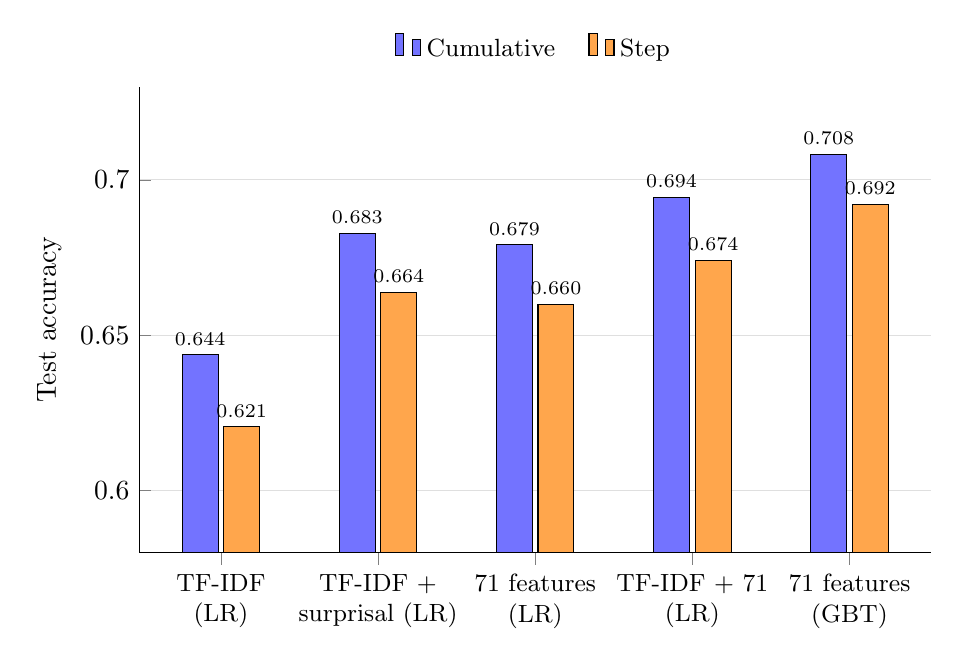
\begin{tikzpicture}
\begin{axis}[
  ybar, bar width=13pt, width=0.96\textwidth, height=7.5cm,
  ymin=0.58, ymax=0.73, ylabel={Test accuracy},
  symbolic x coords={a,b,c,d,e},
  enlarge x limits=0.13,
  xtick=data,
  xticklabels={TF-IDF\\(LR), TF-IDF +\\surprisal (LR), 71 features\\(LR), TF-IDF + 71\\(LR), 71 features\\(GBT)},
  x tick label style={font=\small, align=center},
  yticklabel style={/pgf/number format/fixed, /pgf/number format/precision=2},
  legend style={at={(0.5,1.03)}, anchor=south, legend columns=2, font=\small, draw=none, /tikz/every even column/.append style={column sep=1em}},
  nodes near coords, nodes near coords style={font=\scriptsize, /pgf/number format/fixed, /pgf/number format/precision=3, /pgf/number format/fixed zerofill},
  ymajorgrids, grid style={gray!25}, axis lines*=left]
\addplot[fill=blue!55] coordinates {(a,0.6437) (b,0.6828) (c,0.6791) (d,0.6944) (e,0.7081)};
\addplot[fill=orange!70] coordinates {(a,0.6205) (b,0.6637) (c,0.6600) (d,0.6740) (e,0.6921)};
\legend{Cumulative, Step}
\end{axis}
\end{tikzpicture}
\caption[Accuracy of the main models on pair sheets]{Test accuracy of the main models on the cumulative and step pair sheets (paragraph level). LR: logistic regression; GBT: gradient-boosted trees.}
\label{fig:summary}
\end{figure}

\section{Experiment II-5: Paragraph versus Sentence}
\subsection{Design}
To answer RQ4, the four feature sets of Experiment~II-2 were trained separately on the paragraph and sentence sheets, using the same models, settings and test articles. This comparison isolates TF-IDF, surprisal and MDL; the full-feature models were also run at both levels and are reported in Experiments~II-3 and II-4. As a consistency check, the paragraph results were confirmed to match Experiment~II-2 exactly.

\subsection{Results}
\begin{table}[ht]
\centering
\small
\caption[Experiment II-5: paragraph versus sentence]{Experiment II-5: accuracy (and AUC) at paragraph and sentence level with identical test articles. $\Delta$ = gain over TF-IDF only, in percentage points. Training/test pairs: paragraph cumulative 141{,}322/38{,}673, step 141{,}354/38{,}686; sentence cumulative 149{,}540/41{,}163, step 149{,}571/41{,}176.}
\label{tab:exp5}
\begin{tabular}{@{}llcccc@{}}
\toprule
 & & \multicolumn{2}{c}{Paragraph} & \multicolumn{2}{c}{Sentence}\\
\cmidrule(lr){3-4}\cmidrule(lr){5-6}
Sheet & Feature set & Acc. (AUC) & $\Delta$ & Acc. (AUC) & $\Delta$\\
\midrule
\multirow{4}{*}{Cumulative} & TF-IDF & 0.644 (0.718) & -- & 0.604 (0.666) & --\\
 & + surprisal & 0.683 (0.744) & $+3.91$ & 0.660 (0.719) & $\mathbf{+5.56}$\\
 & + MDL & 0.644 (0.718) & $+0.06$ & 0.606 (0.667) & $+0.12$\\
 & + both & 0.683 (0.744) & $+3.97$ & 0.660 (0.720) & $+5.56$\\
\midrule
\multirow{4}{*}{Step} & TF-IDF & 0.620 (0.685) & -- & 0.597 (0.655) & --\\
 & + surprisal & 0.664 (0.716) & $+4.32$ & 0.654 (0.711) & $\mathbf{+5.73}$\\
 & + MDL & 0.620 (0.686) & $-0.06$ & 0.598 (0.655) & $+0.08$\\
 & + both & 0.663 (0.717) & $+4.29$ & 0.653 (0.711) & $+5.64$\\
\midrule
\multirow{4}{*}{Absolute} & TF-IDF & 0.545 (0.576) & -- & 0.547 (0.578) & --\\
 & + surprisal & 0.545 (0.575) & $+0.03$ & 0.553 (0.586) & $+0.62$\\
 & + MDL & 0.545 (0.576) & $+0.04$ & 0.547 (0.577) & $-0.04$\\
 & + both & 0.545 (0.576) & $+0.04$ & 0.554 (0.586) & $+0.66$\\
\bottomrule
\end{tabular}
\end{table}

\begin{figure}[ht]
\centering
\safefig{figures/exp5-paragraph-vs-sentence.png}{\textwidth}
\caption[Paragraph versus sentence accuracy (Experiment II-5)]{Paragraph (blue) versus sentence (orange) accuracy for each feature set (top) and the gain over TF-IDF only (bottom), for the absolute, cumulative and step sheets.}
\label{fig:exp5}
\end{figure}

Table~\ref{tab:exp5} and Figure~\ref{fig:exp5} show two opposite effects. In absolute terms, sentence pairs are \emph{harder} to classify: TF-IDF alone drops from 64.4\% to 60.4\% on cumulative pairs because a single sentence offers far fewer words for the model to use. But the \emph{added value} of surprisal is larger at sentence level, $+5.6$ and $+5.7$ points against $+3.9$ and $+4.3$ at paragraph level. Surprisal is also the only feature that lifts the absolute sheet noticeably at sentence level ($+0.6$ points). MDL contributes nothing at either level. This matches Experiment~I. When the unit of analysis is the sentence that was actually edited, the surprisal signal is not diluted by unchanged neighbouring sentences.

The full-feature models narrow the gap between the two levels without closing it. TF-IDF alone is 3.9 points worse at sentence level on cumulative pairs and 2.4 points worse on step pairs. With TF-IDF plus all selected features the gap is 2.8 and 1.4 points (Tables~\ref{tab:exp3} and \ref{tab:exp3-sent}), and for the gradient-boosted trees it is 3.3 and 2.7 points (Table~\ref{tab:exp4}). The linguistic profile therefore makes up for that part but not all of the information lost when the model sees one sentence instead of a whole paragraph.

\section{Summary of Experiment II}
\begin{itemize}
  \item \textbf{RQ2.} GPT-2 surprisal is by far the most useful surprisal measure. It adds about 4 points of accuracy over TF-IDF, three times as much as the best $n$-gram model.
  \item \textbf{RQ3.} Surprisal carries information about the direction of an edit that word features do not. MDL adds nothing on its own but receives a negative weight once other features are controlled for. The best model, gradient-boosted trees over 71 linguistic features, reaches 70.8\% accuracy (AUC 0.782) on cumulative pairs.
\item \textbf{RQ4.} The surprisal gain is larger at sentence level than at paragraph level, although sentence pairs are harder overall. With all 69 sentence-level features, the best sentence model (gradient-boosted trees) reaches 67.5\% accuracy (AUC 0.751) on cumulative pairs and GPT-2 surprisal is the strongest feature in the sentence-level linear model.
\end{itemize}

%% =====================================================================
%%  CHAPTER 6 -- DISCUSSION
%% =====================================================================
\chapter{Discussion}
\label{ch:discussion}

This chapter interprets the results of the two experiments, relates them to the theories introduced in Chapter~\ref{ch:background}, and describes the limitations that should be kept in mind.

\section{Revision Makes Text More Predictable}
The most consistent finding of this thesis is that collaborative revisions of wikiHow text tend to lower its surprisal under a contextual language model. The effect appears in both experiments. Descriptively, a majority of edits reduce surprisal, the median change is negative at every depth, and the cumulative reduction becomes larger the more often a paragraph is revised. Predictively, surprisal is the single most useful feature beyond the words themselves, and it keeps a large weight when seventy other features are present.

This is what expectation-based theories of processing predict for text that is being optimised for readers. If reading effort grows with surprisal, as expectation based theories assume \citep{hale2001}, then lowering mean surprisal by a few tenths of a bit per token, as seen in heavily revised paragraphs, means a lower expected processing cost per word. The steady shrinking of the positive tail with depth (Figure~\ref{fig:gpt2-depth}) suggests that later edits are especially likely to remove surprisal peaks rather than add them.

The effect is a tendency, not a rule. About 44\% of edits increase surprisal and many of them are large. Not every revision aims at readability. Contributors also add missing information, correct facts and insert warnings and such edits naturally add unexpected content. The fact that the mean is sometimes positive while the median is negative reflects this mixture i.e. a majority of small, smoothing edits combined with a minority of larger, content-adding ones.

\section{Why GPT-2 and $n$-gram Surprisal Disagree}
One of the most striking results is that $n$-gram models report the \emph{opposite} trend to GPT-2. Three differences between the models explain why.

\paragraph{Context.} An $n$-gram model looks at most four words back, while GPT-2 conditions on the whole preceding paragraph. Many revisions improve the coherence between sentences, for instance by naming the key object again where a vague pronoun stood before, or by stating a topic before referring to it. These changes reduce surprisal only for a model that can see the earlier sentence.

\paragraph{Domain.} The $n$-gram models were trained on newswire, encyclopaedic and general corpora, none of which contain instructional text. Revisions to wikiHow often replace general words with specific ones (brand names, measurements, interface labels). These words are rare or unknown in the reference corpora, so the $n$-gram models give them high surprisal. GPT-2 was trained on a much larger and more varied web corpus and handles such vocabulary better.

\paragraph{Model quality.} GPT-2 is a far stronger language model than the $n$-gram models as it was trained on much more text and conditions on a longer context. Its probability estimates are therefore likely to be closer to what a human reader experiences and the $n$-gram trend is more likely an artefact of the mismatch between those models and the domain.

Experiment~II-1 confirms this reading independently. GPT-2 surprisal is far more useful for prediction, and the GPT-2 and $n$-gram measures are only weakly to moderately correlated with each other (Pearson $r$ between 0.25 and 0.53 at paragraph level and between 0.18 and 0.49 at sentence level, over all twelve corpus and order combinations checked). The methodological lesson is that conclusions about surprisal in a specialised genre can depend on the language model used to estimate it, and that cross model checks such as the one reported here are worth carrying out.

\section{Why Dependency Length Does Not Fall}
The null result for MDL needs careful interpretation. It does not show that dependency locality is irrelevant to revision. Four considerations suggest a more limited conclusion.

First, many edits do not change syntax at all. Between 20\% and 30\% of edits leave MDL exactly unchanged because they correct spelling, replace a word or change punctuation. Dependency locality can only matter for edits that restructure a sentence, and those are a minority.

Second, wikiHow sentences tend to be short and simple. Steps usually open with an imperative clause and in short sentences dependency lengths are already close to their minimum, leaving little room to shorten them further.

Third, the length of the text is a confound. Revisions often add clauses, conditions and examples. Longer sentences have longer dependencies on average, so any local reordering that reduces dependency length can be outweighed by added material. The negative MDL coefficient in the multivariate model of Experiment~II-3, where sentence length and diversity are controlled for supports this explanation at paragraph level is once these are held constant, a lower MDL does point towards the revised version. The same effect is not found at sentence level however, so this explanation remains tentative.

Fourth, MDL is a sentence level average and may be too coarse. An edit that shortens a single long dependency in a ten-arc sentence changes the mean only slightly. Measures focused on the longest dependency, or measures that take sentence length into account, may be more sensitive.

\section{Granularity}
The comparison between paragraphs and sentences shows that the unit of analysis matters. Paragraph level measures average over sentences that an edit did not touch, so the signal is diluted. Sentence alignment isolates the part that changed and gives the clearest evidence of surprisal reduction. Paragraph level models still classify more accurately overall, because they have more words to work with and with the full feature set the best paragraph model is 3.3 points more accurate than the best sentence model. A practical system for detecting or suggesting revisions could therefore combine the two levels, using paragraph context to judge an edit as a whole and sentence level surprisal to locate the part that changed.

\section{Relation to Prior Work on wikiHow}
\citet{anthonio2020} showed that original and revised wikiHow sentences can be told apart with text classifiers. The present results agree with theirs and add an explanation of \emph{what} distinguishes the two. Part of the signal lies in predictability, a quantity that expectation-based theory links to processing effort \citep{hale2001}. The best model here uses interpretable features, and its performance is not directly comparable to that study which used a different corpus construction, sentence level data and different models. The two lines of work should be seen as complementary rather than competing.

\section{Limitations}
Several limitations qualify these conclusions.
\begin{itemize}
  \item \textbf{Proxies, not readers.} Surprisal and MDL are model-based proxies for cognitive load. No reading-time, eye-tracking or comprehension data were collected for the revised texts, so the claim that revisions reduce \emph{human} effort is inferred, not measured.
  \item \textbf{Coverage.} Histories were collected for 66\% of catalogued articles. If the missing articles differ systematically, for example by being older or more heavily edited, the corpus may not be fully representative of wikiHow.
  \item \textbf{Filtering choices.} The BLEU threshold, the revert window and the junk rules were set by inspection. Different settings would change which edits are kept, especially edits that rewrite large parts of a paragraph, which the BLEU filter is most likely to remove.
  \item \textbf{No edit-type labels.} All edits are treated alike. The effect is mostly concentrated in stylistic and clarifying base edits and absent from factual updates but the corpus does not contain the labels needed to test this directly.
  \item \textbf{Selection by depth.} Paragraphs that are revised many times are not a random sample, so the depth trends describe what happens to such paragraphs and should not be read as the causal effect of extra edits.
  \item \textbf{Single language model family.} Only GPT-2 small was used for neural surprisal. Larger models, or models adapted to instructional text, might change the size of the effect.
\item \textbf{Single split.} All classifiers use one fixed article level split. Although the test set is large (over 38{,}000 pairs), confidence intervals from repeated splits or bootstrapping were not computed.
\end{itemize}

\section{Ethical Considerations}
The data consist of publicly visible article text and edit histories. Only article content was used. No contributor names, user profiles or other personal information were stored or analysed. The scraper limited its request rate to avoid placing unnecessary load on the website. The corpus is intended for research use and is not redistributed with this thesis.

%% =====================================================================
%%  CHAPTER 7 -- CONCLUSION
%% =====================================================================
\chapter{Conclusion}
\label{ch:conclusion}

\section{Summary}
This thesis asked whether the collaborative revision of instructional text reduces the cognitive load that the text places on its readers, measured through surprisal and dependency length. To answer this, it built a corpus of 180{,}536 paragraph edits and 191{,}359 sentence edits from the revision histories of 7{,}519 wikiHow articles. It extracted 112 linguistic measures for every version and carried out one descriptive and five predictive experiments.

The answers to the four research questions are as follows.
\begin{enumerate}[label=\textbf{RQ\arabic*.},leftmargin=*]
  \item Revisions tend to make text more predictable. Around 56\% of edits lower GPT-2 surprisal, the median change is negative at every depth, and the reduction relative to the original grows to about 0.3 bits per token for repeatedly revised paragraphs. Mean dependency length does not fall in the raw data and rises slightly as paragraphs grow.
  \item Which way surprisal moves is partly a property of the model that measures it. GPT-2 detects the reduction, while $n$-gram models estimated from non-wikiHow corpora show a small increase. GPT-2 surprisal is also three times as useful for prediction as the best $n$-gram variant.
  \item Surprisal adds about four points of accuracy over a strong lexical baseline for telling an original from its revision, while MDL adds nothing on its own. A non-linear model over 71 interpretable features reaches 70.8\% accuracy and 0.782 AUC.
\item The surprisal signal is stronger for sentences compared to paragraphs, even though sentence pairs are harder to classify overall. At sentence level, surprisal adds about 5.6 points over the lexical baseline, it is the strongest of all 69 features in the full linear model and the best model reaches 67.5\% accuracy and 0.751 AUC.
\end{enumerate}

Overall, the evidence supports the view that people who revise instructional text, whether or not they intend it, move it towards forms that a predictive reader would find easier. The evidence is clearer for predictability than for syntactic locality.

\section{Future Work}
Several directions follow naturally from this study.
\begin{itemize}
  \item \textbf{Human validation.} A reading-time or comprehension study on a sample of original/revised pairs would test directly whether the reduction in model surprisal corresponds to reduced human effort.
  \item \textbf{Edit-type analysis.} Labelling a sample of edits by intention (clarification, elaboration, correction, formatting) would show which kinds of edit drive the surprisal reduction, and would allow the analysis to be restricted to edits aimed at readability.
  \item \textbf{Better locality measures.} Comparing observed dependency lengths with random or optimal linearisations of the same tree, or examining only edits that reorder words, would give a sharper test of whether revisers shorten dependencies.
  \item \textbf{Stronger and adapted language models.} Repeating the analysis with larger language models, and with models fine-tuned on instructional text, would show how robust the surprisal effect is and whether domain adaptation reduces the disagreement between models.
  \item \textbf{Revision assistance.} The trained pair models already power a small interactive demonstration that scores two versions of a paragraph. Extending it into a tool that highlights high-surprisal spans and proposes alternatives would turn the findings into practical support for writers.
  \item \textbf{Other genres and languages.} Applying the same pipeline to Wikipedia or to wikiHow in other languages would show whether the pattern is specific to instructional English or a general property of collaborative revision.
\end{itemize}

%% =====================================================================
%%  REFERENCES
%% =====================================================================
\begin{thebibliography}{99}
\addcontentsline{toc}{chapter}{References}
\small

\bibitem[Hale(2001)]{hale2001}
J.~Hale, ``A probabilistic Earley parser as a psycholinguistic model,'' in \emph{Proc. 2nd Meeting of the North American Chapter of the Association for Computational Linguistics (NAACL)}, 2001.

\bibitem[Gibson(1998)]{gibson1998}
E.~Gibson, ``Linguistic complexity: Locality of syntactic dependencies,'' \emph{Cognition}, vol.~68, no.~1, 1998.

\bibitem[Anthonio et~al.(2020)]{anthonio2020}
T.~R. Anthonio, I.~Bhat, and M.~Roth, ``wikiHowToImprove: A resource and analyses on edits in instructional texts,'' in \emph{Proc. 12th Language Resources and Evaluation Conference (LREC)}, 2020.

\bibitem[Kazmi et~al.(2022)]{kazmi2022}
A.~Kazmi, S.~Ranjan, A.~Sharma, and R.~Rajkumar, ``Linguistically motivated features for classifying shorter text into fiction and non-fiction genre,'' in \emph{Proc. 29th International Conference on Computational Linguistics (COLING)}, 2022.

\bibitem[Faruqui et~al.(2018)]{faruqui2018}
M.~Faruqui, E.~Pavlick, I.~Tenney, and D.~Das, ``WikiAtomicEdits: A multilingual corpus of Wikipedia edits for modeling language and discourse,'' in \emph{Proc. Conference on Empirical Methods in Natural Language Processing (EMNLP)}, 2018.

\bibitem[Daxenberger and Gurevych(2013)]{daxenberger2013}
J.~Daxenberger and I.~Gurevych, ``Automatically classifying edit categories in Wikipedia revisions,'' in \emph{Proc. Conference on Empirical Methods in Natural Language Processing (EMNLP)}, 2013.

\bibitem[Radford et~al.(2019)]{radford2019}
A.~Radford, J.~Wu, R.~Child, D.~Luan, D.~Amodei, and I.~Sutskever, ``Language models are unsupervised multitask learners,'' OpenAI, Tech. Rep., 2019.

\bibitem[Papineni et~al.(2002)]{papineni2002}
K.~Papineni, S.~Roukos, T.~Ward, and W.-J. Zhu, ``BLEU: A method for automatic evaluation of machine translation,'' in \emph{Proc. 40th Annual Meeting of the Association for Computational Linguistics (ACL)}, 2002.

\bibitem[Chen and Cherry(2014)]{chen2014}
B.~Chen and C.~Cherry, ``A systematic comparison of smoothing techniques for sentence-level BLEU,'' in \emph{Proc. 9th Workshop on Statistical Machine Translation}, 2014.

\bibitem[Honnibal et~al.(2020)]{honnibal2020}
M.~Honnibal, I.~Montani, S.~Van~Landeghem, and A.~Boyd, ``spaCy: Industrial-strength natural language processing in Python,'' Zenodo, 2020.

\bibitem[Stolcke(2002)]{stolcke2002}
A.~Stolcke, ``SRILM -- An extensible language modeling toolkit,'' in \emph{Proc. 7th International Conference on Spoken Language Processing (ICSLP)}, 2002.

\bibitem[Francis and Ku\v{c}era(1979)]{francis1979}
W.~N. Francis and H.~Ku\v{c}era, \emph{Brown Corpus Manual}. Providence, RI, USA: Department of Linguistics, Brown University, 1979.

\bibitem[Marcus et~al.(1993)]{marcus1993}
M.~P. Marcus, B.~Santorini, and M.~A. Marcinkiewicz, ``Building a large annotated corpus of English: The Penn Treebank,'' \emph{Computational Linguistics}, vol.~19, no.~2, 1993.

\bibitem[Merity et~al.(2017)]{merity2017}
S.~Merity, C.~Xiong, J.~Bradbury, and R.~Socher, ``Pointer sentinel mixture models,'' in \emph{Proc. International Conference on Learning Representations (ICLR)}, 2017.

\bibitem[Pedregosa et~al.(2011)]{pedregosa2011}
F.~Pedregosa, G.~Varoquaux, A.~Gramfort \emph{et~al.}, ``Scikit-learn: Machine learning in Python,'' \emph{Journal of Machine Learning Research}, vol.~12, 2011.

\bibitem[Friedman(2001)]{friedman2001}
J.~H. Friedman, ``Greedy function approximation: A gradient boosting machine,'' \emph{The Annals of Statistics}, vol.~29, no.~5, 2001.

\end{thebibliography}

%% =====================================================================
%%  APPENDICES
%% =====================================================================
\appendix

\chapter{Feature Inventory}
\label{app:features}
Table~\ref{tab:inventory} lists the 112 candidate measures by family. The features retained after filtering (71 at paragraph level, 69 at sentence level) are saved by the dataset-building notebook in the file \nolinkurl{feature-engineering/final_features.csv}.

\begin{table}[ht]
\centering
\small
\caption{Candidate measures computed for every version.}
\label{tab:inventory}
\begin{tabularx}{\textwidth}{@{}lrX@{}}
\toprule
Family & Count & Measures\\
\midrule
Raw & 2 & mean and standard deviation of sentence length\\
Lexical & 17 & TTR, Maas TTR, MSTTR, MATTR, MTLD, MTLD-MA, vocd-D, Yule's $K$ (character and word level); lexical density\\
POS ratios & 8 & adv/noun, adv/pron, adj/verb, noun/verb, verb/pron, adv/adj, adj/pron, noun/pron\\
Syntactic & 63 & tree depth, ISC, argument/adjunct ratio, relative frequency of UD relations, directional head--dependent POS bigrams\\
Dependency length & 1 & mean dependency length (MDL)\\
GPT-2 surprisal & 1 & mean token surprisal, sentence-averaged\\
$n$-gram surprisal & 20 & 4 corpora (Brown, PTB-WSJ, WikiText-2, Simple Wikipedia) $\times$ orders 1--5\\
\midrule
Total & 112 & \\
\bottomrule
\end{tabularx}
\end{table}

\chapter{Implementation and Reproducibility}
\label{app:repro}
The project is organised as three self-contained folders that are run in order.
{\raggedright
\begin{description}[style=nextline, leftmargin=1.5em]
  \item[\texttt{data-collection/}] Sitemap crawler, history scraper and bundler; produces \texttt{edit\_history.jsonl.gz}.
  \item[\texttt{data-preprocessing/}] Eight pipeline stages (\texttt{python -m pipeline.run\_all}); stages 2--7 can be run for one article with \texttt{-{}-article}. Produces \texttt{revision\_groups.jsonl.gz}.
  \item[\texttt{experiments/}] Jupyter notebooks in five numbered folders: data preparation, feature extraction, dataset building, analysis and models. Every notebook has a \texttt{LEVEL} switch (\texttt{"paragraph"} or \texttt{"sentence"}).
\end{description}
\par}

\paragraph{Software.} Python 3.12; spaCy with \texttt{en\_core\_web\_trf}; Hugging Face Transformers with GPT-2 small; SRILM for $n$-gram training and scoring; NLTK for BLEU; \texttt{lexicalrichness} for lexical diversity; scikit-learn for TF-IDF, logistic regression and histogram gradient boosting; pandas, NumPy and Matplotlib for analysis and plotting.

\paragraph{Key settings.} Random seed 42; test share 20\% of articles; BLEU threshold 0.06 (paragraph filter and sentence-group split); revert window 5; TF-IDF word 1--2-grams, \texttt{min\_df}=2, at most 20{,}000 features; logistic regression \texttt{max\_iter}=2000; gradient boosting learning rate 0.1, at most 500 iterations, early stopping; correlation threshold $|r|>0.90$; undefined-value threshold 5\%.

\paragraph{Demonstration.} A small Streamlit application loads the trained paragraph-level pair models and, given two versions of a paragraph, reports which one the models consider to be the revision.

\end{document}
